
\documentclass[11pt]{article}

\usepackage[T1]{fontenc}
\usepackage[utf8]{inputenc}
\usepackage{lmodern}
\usepackage[margin=1in]{geometry}
\usepackage{graphicx}
\usepackage{booktabs}
\usepackage{amsmath}
\usepackage{authblk}
\usepackage[labelsep=period]{caption}
\usepackage{xcolor}
\usepackage[hidelinks]{hyperref}
\usepackage[numbers,sort&compress]{natbib}

\emergencystretch=2em

\newcommand{\pstatone}{pY-STAT1}
\newcommand{\pstatthree}{pY-STAT3}
\newcommand{\logmean}{log-mean}
\newcommand{\icfifty}{IC$_{50}$}
\newcommand{\ifng}{IFN-$\gamma$}

\title{Single-cell profiling quantifies the dose gap between population-average and complete pY-STAT1/3 suppression by JAK inhibitors}

\author[1]{Karolina Ewa Zakrzewska$^\dagger$}
\author[1]{Jaros{\l}aw Walczak$^{\dagger}$}
\author[1]{Karol Niena{\l}towski}
\author[1]{Piotr Topolewski}
\author[3]{Christina Maria Wagner}
\author[2]{Agata Braniewska}
\author[2]{Tomasz Rygiel}
\author[3]{Richard Moriggl}
\author[1,*]{Micha{\l} Komorowski}

\affil[1]{Institute of Fundamental Technological Research, Polish Academy of Sciences, Warsaw, Poland}
\affil[2]{Department of Immunology, Mossakowski Medical Research Institute, Polish Academy of Sciences, Warsaw, Poland}
\affil[3]{Institute of Animal Breeding and Genetics, University of Veterinary Medicine, Vienna, Austria}
\affil[*]{Correspondence: m.komorowski@sysbiosig.org}

\date{}

\begin{document}
\maketitle

\begin{center}
$^\dagger$ These authors contributed equally to this work.
\end{center}

\begin{abstract}
Inhibitor potency is commonly assessed from population-average responses, but how much single-cell signaling remains under strong average suppression is less clear. We measured nuclear STAT1 and STAT3 tyrosine phosphorylation in two human monocytic cell lines stimulated with \ifng{} and IL-10 and treated with six JAK-pathway inhibitors. Across 24 profiles, we compared arithmetic-mean inhibition and inhibition of the mean of log10-transformed single-cell responses (log-mean) with the fractions of cells leaving the stimulated range (partial inhibition) or entering the non-stimulated range (complete inhibition). At the lowest tested doses where arithmetic-mean or log-mean inhibition reached at least 80\%, median fractions remaining above the non-stimulated range were 76\% and 37\%, respectively. Thus, strong average suppression frequently left substantial fractions of cells with tangibly elevated pY-STAT responses. Log-mean inhibition generally approximated partial-inhibition occupancy, whereas the apparent \icfifty{} for complete-inhibition occupancy was a median 2.4-fold higher than the log-mean \icfifty{} and 7.4-fold higher than the arithmetic-mean \icfifty{}. These relationships provide an empirical guide for estimating cell fractions from conventional inhibition curves.
\end{abstract}

\noindent\textbf{Keywords:} single-cell signaling; JAK-STAT; heterogeneity; inhibitor profiling; IC50; population summary

\section*{Introduction}
Signaling pathways translate extracellular cues into cellular responses and are major pharmacological targets in the treatment of diverse diseases \citep{behar2013dynamics,yi2024targeting}. Yet cells exposed to the same stimulus can respond very differently \citep{irish2004single,gabor2021cell}. In cytokine signaling, single-cell responses span broad, overlapping distributions \citep{nienaltowski2021fractional,topolewski2022phenotypic}. This variability can reflect differences in molecular content and cellular state, as well as biochemical noise \citep{altschuler2010cellular,niepel2009non,topolewski2022phenotypic}.

Cells also differ in their responses to inhibitors \citep{krutzik2008high,bodenmiller2012multiplexed}. At the same drug concentration, signaling may be strongly suppressed in some cells while remaining elevated in others \citep{kinnunen2024characterizing}. Inhibition can also take different forms: increasing drug concentration may progressively lower the signal in responding cells or reduce the fraction of responding cells while leaving the remaining responders relatively unaffected \citep{vogel2016dichotomy}. These patterns distinguish two aspects of inhibitor action: how much signaling is reduced within cells and how many cells are affected.

This raises a practical question: how should responses to stimulation and inhibition be quantified? Population averages are convenient and widely used summaries, but they need not capture the features of a response distribution that matter most for a particular biological outcome \citep{gough2017biologically}. Small cell subsets can shape immune responses \citep{satija2014heterogeneity,shalek2014single}, and non-genetic differences among cells can contribute to incomplete responses to drug treatment \citep{niepel2009non,aissa2021singlecell}. Drug-response studies also show that potency alone does not fully describe inhibitor effects \citep{fallahi2013metrics}. For instance, in proliferation assays, conventional potency estimates can also depend on how many cell divisions occur during treatment \citep{hafner2016growth}. A useful description of inhibition therefore needs to consider not only the average response, but also how responses are distributed across cells \citep{lun2020profiling}.

The relationship between signaling and downstream function can be complex and context-dependent \citep{cui2024dictionary}, so no single signaling metric can be assumed to predict every biological outcome. For example, IL-6 and IL-10 both activate STAT3 in human dendritic cells, yet differences in the duration of activation help explain their contrasting inflammatory effects \citep{braun2013cytokine}. Compounds nevertheless need to be, and often are,  characterized even when this relationship has not yet been established. In this setting, experimentally measured reference distributions offer a simple basis for assessing inhibition while accounting for cell-to-cell heterogeneity: how many cells leave the fully stimulated response range, and how many enter the non-stimulated range? These criteria mark two ends of the reference-defined response shift and complement population averages without presuming which measure best predicts function.  Because inhibitor effects are commonly reported as population-average curves \citep{mcinnes2019comparison}, an empirical link to reference-based cell fractions would help interpret what a given level of average suppression means for individual cells. We therefore asked what fractions of cells typically leave the stimulated range or enter the non-stimulated range at a given level of population inhibition, and how much these fractions vary across biological and pharmacological conditions.

We examined these relationships in cytokine-induced JAK-STAT signaling, using nuclear STAT1 phosphorylated at Tyr701 (\pstatone{}) and STAT3 phosphorylated at Tyr705 (\pstatthree{}) as readouts. We defined state occupancy as the fraction of cells within a predefined response range. We compared partial- and complete-inhibition occupancy with inhibition of the arithmetic mean and of the mean of log10-transformed single-cell responses, hereafter log-mean.

JAK-inhibitor profiling in human blood has shown that apparent potency varies with the cytokine stimulus, pY-STAT readout, and cell type \citep{traves2021jak}. We therefore examined how the relationship between population inhibition and state occupancy varies across six inhibitors in two human monocytic cell lines, THP-1 and U937. The panel combined solcitinib, BMS-911543, and the dual SYK/JAK inhibitor cerdulatinib, which have different reported target profiles, with three clinically used JAK inhibitors with overlapping JAK-family activity: baricitinib, ruxolitinib, and tofacitinib \citep{haikarainen2026pharmacological,wan2015discovery,ma2015cerdulatinib}. This design allowed us to assess both the typical relationship between average inhibition and cell fractions and its variation across experimental conditions.


Across the tested panel, we quantified how arithmetic-mean and log-mean inhibition relate to the fractions of cells leaving the stimulated range or entering the non-stimulated range. Log-mean inhibition generally approximated departure from the stimulated range, whereas complete-inhibition occupancy was shifted toward higher inhibitor concentrations. The apparent \icfifty{} for complete-inhibition occupancy was a median 2.4-fold higher than the log-mean \icfifty{} and 7.4-fold higher than the arithmetic-mean \icfifty{}. Together, these comparisons provide an empirical guide to the cell fractions associated with a given level of average suppression, including the fraction retaining elevated pY-STAT responses, and show how much these relationships vary across biological and pharmacological conditions.

\section*{Results}

\subsection*{Single-cell response distributions motivate state-occupancy metrics}

To motivate a state-occupancy approach to quantifying inhibitor effects, we first examined representative single-cell distributions of \pstatone{} and \pstatthree{} under cytokine stimulation and JAK inhibition (Figure~\ref{fig:fig1}). Panel A shows response distributions at selected cytokine concentrations for \ifng{}-induced \pstatone{} and IL-10-induced \pstatthree{} \citep{bhat2018comprehensive,verma2016network}, together with the combined full-stimulation reference used in the inhibition experiments.

Panel B defines the non-stimulated and fully stimulated reference distributions used to set state-occupancy thresholds. Panel C shows how inhibitor-treated distributions are redistributed by increasing concentrations of a representative inhibitor, cerdulatinib, and Panel D summarizes the same redistribution as state occupancy. Responses are plotted on the log-response axis, on which the breadth and overlap of the distributions are most readily visualized.

Two features of these distributions motivate the subsequent analysis. First, the distributions are broad and overlapping: cells exposed to different cytokine concentrations can exhibit similar responses, and even under strong stimulation a fraction of cells remains close to the low-response range. Stimulation therefore redistributes cells across a broad range of responses rather than simply shifting a single characteristic response. Second, the form of this redistribution differs between the two readouts. For \pstatone{}, increasing \ifng{} concentration produces a predominantly graded response, with the distribution shifting progressively toward higher values. For \pstatthree{}, increasing IL-10 concentration broadens and flattens the distribution over the examined range, indicating that dose affects both the fraction of cells with elevated \pstatthree{} and the response magnitude among those cells. These patterns show that a population summary alone cannot specify how inhibitor treatment redistributes cells among distinct response ranges.

Panels B--D introduce the state-occupancy metrics used throughout the manuscript. The complete-inhibition threshold is defined by the 95th percentile of the non-stimulated reference distribution. Cells below this threshold are assigned to the complete-inhibition state. The partial-inhibition threshold is defined by the 5th percentile of the fully stimulated reference distribution, constrained not to fall below the complete threshold when the references overlap (Methods). Partial-inhibition occupancy is the fraction of cells below this threshold and therefore includes both cells in the complete-inhibition state and cells in the intermediate range between the two thresholds. In Figure~\ref{fig:fig1}, blue denotes the complete-inhibition range, red the intermediate partial-only range, and gray responses above the partial-inhibition threshold. Red and gray together constitute the residual pY-STAT-positive fraction.

The cerdulatinib-treated distributions show increasing occupancy of the intermediate partial-only range as concentration rises, followed by greater occupancy of the non-stimulated range at higher doses. These are comparisons of cell populations at a fixed endpoint, not trajectories of the same cells. The histograms and stacked occupancy bars show why strong attenuation of a population-level response can coexist with limited occupancy of the non-stimulated range.

\subsection*{Representative inhibition curves separate population suppression from complete-inhibition occupancy}

Representative THP-1 dose-response profiles illustrate why population suppression and state occupancy cannot be treated as equivalent pharmacological endpoints (Figure~\ref{fig:fig2}). Each panel overlays arithmetic-mean inhibition, log-mean inhibition, partial-inhibition occupancy, and complete-inhibition occupancy. Solcitinib and cerdulatinib were selected because together they show the principal relationships among these endpoints for both \pstatone{} and \pstatthree{}; the corresponding curves for all inhibitors, cell lines, and readouts are shown in Supplementary Figure~\ref{fig:figs1}.

Across all four panels, arithmetic-mean inhibition is left-shifted relative to log-mean inhibition, indicating lower apparent inhibitory concentrations when responses were averaged on the raw scale. Complete-inhibition occupancy is generally displaced furthest to the right. Partial-inhibition occupancy remains closer to the population summaries than complete-inhibition occupancy, consistent with all three endpoints being influenced by the bulk of the responding distribution. Although the precise ordering of the endpoints varies among conditions, the curves consistently show that attenuation of the typical response and entry into the complete-inhibition state can occur at different inhibitor concentrations.

This separation is particularly clear for cerdulatinib-inhibited \pstatone{} (Figure~\ref{fig:fig2}C). At intermediate concentrations, arithmetic-mean inhibition is close to saturation, and both log-mean inhibition and partial-inhibition occupancy are high, yet complete-inhibition occupancy remains low. The population response can therefore be strongly attenuated while many cells remain above the non-stimulated range. A similar separation is visible for solcitinib-inhibited \pstatthree{} (Figure~\ref{fig:fig2}B), where both population summaries indicate substantial inhibition before complete-inhibition occupancy rises appreciably.

These examples show that the discrepancy is not restricted to the known difference between arithmetic averaging and analysis on the log-response scale. The log-mean provides a less left-shifted population benchmark than the arithmetic mean, but it still does not specify how many cells have entered the non-stimulated response range. The following analysis tests how consistently this separation occurs across the full inhibitor--cell-line--readout panel.

\subsection*{Matching population inhibition to state occupancy reveals residual pY-STAT-positive fractions}

We next used the full inhibitor--cell-line--readout panel to establish the empirical relationship between population inhibition and single-cell state occupancy. Across 24 profiles, Figure~\ref{fig:fig3} asks what fractions of cells had left the fully stimulated response range or entered the complete-inhibition state at matched levels of arithmetic-mean or log-mean inhibition. This comparison quantifies both how informative a population-inhibition curve is about the underlying redistribution of single-cell responses and how large a residual pY-STAT-positive fraction may remain.

Partial-inhibition occupancy remained relatively close to both population summaries across doses (Figure~\ref{fig:fig3}A,B). At the lowest measured dose at which fitted log-mean inhibition reached each benchmark (0.2, 0.5, or 0.8), median partial-inhibition occupancy was 0.28, 0.61, and 0.89, respectively (Figure~\ref{fig:fig3}C,D). The log-mean therefore provided a close, although not exact, benchmark for the fraction of cells that had left the fully stimulated response range. The remaining profile-to-profile differences were structured: variance partitioning identified phospho-target as the largest identifiable contributor in most threshold--summary combinations and on average (Figure~\ref{fig:fig3}E).

Complete-inhibition occupancy was more loosely related to population inhibition. Across the same profiles, the fraction of cells entering the non-stimulated response range was generally lower than the corresponding population-summary inhibition (Figure~\ref{fig:fig3}F,G). Applying the same lowest-dose criterion across inhibition benchmarks revealed a nonlinear relationship. At arithmetic-mean inhibition levels of 0.2, 0.5, and 0.8, median complete-inhibition occupancy was 0.02, 0.05, and 0.24, respectively. At the corresponding log-mean inhibition levels, median occupancy was 0.04, 0.20, and 0.63 (Figure~\ref{fig:fig3}H,I). Thus, the log-mean approached complete-inhibition occupancy more closely at high levels of population suppression than did the arithmetic mean. Even at the 0.8 benchmark, however, the discrepancy remained substantial across individual profiles. At the lowest measured dose at which arithmetic-mean inhibition reached 0.8, complete-inhibition occupancy had an interquartile range of 0.07--0.47 and remained below 0.3 in 12 of 23 evaluable profiles. At the corresponding log-mean benchmark, complete-inhibition occupancy remained below 0.5 in 5 of 22 evaluable profiles. Expressed as residual fractions, doses meeting the 80\% arithmetic-mean or log-mean inhibition benchmark still left median residual pY-STAT-positive fractions of 76\% and 37\%, respectively. The log-mean gave a closer approximation to complete-inhibition occupancy than the arithmetic mean, but the same level of population inhibition still corresponded to different cell fractions across conditions.

The residual pY-STAT-positive fraction at matched population inhibition also differed systematically among profiles. Cell line, inhibitor, and phospho-target together accounted for approximately 60--70\% of the between-profile variance in complete-inhibition occupancy at the examined thresholds. Cell line provided the largest identifiable contribution in most configurations and on average (label-permutation test on cell line, $p \le 0.003$; Figure~\ref{fig:fig3}J), whereas 30--40\% of the variance was not explained by the factors included in the analysis. In contrast, the largest identifiable contribution to variation in partial-inhibition occupancy was generally associated with phospho-target rather than cell line (Figure~\ref{fig:fig3}E). These are descriptive associations within this panel: only two cell lines were examined, and batch is confounded with cell line and inhibitor panel (Methods).

Together, these comparisons provide an empirical basis for estimating cell fractions from conventional inhibition curves, including their variation across conditions. We next quantified the corresponding dose gap between population inhibition and state occupancy using apparent \icfifty{} values.

\subsection*{Complete-inhibition occupancy shows a median 2.4-fold dose gap from the log-mean and 7.4-fold from the arithmetic mean}

We next asked how much the estimated inhibitory dose changes when inhibition is assessed by cell fractions rather than population averages. For each of the 24 profiles, we compared the concentrations at the fitted midpoints of the four response curves: the apparent \icfifty{} values for arithmetic-mean inhibition, log-mean inhibition, partial-inhibition occupancy, and complete-inhibition occupancy (Figure~\ref{fig:fig4}).

Partial-inhibition \icfifty{} values lay close to the population-summary estimates, particularly the log-mean (Figure~\ref{fig:fig4}A,B). The median ratio of partial-inhibition \icfifty{} to log-mean \icfifty{} was 0.8 (95\% confidence interval, 0.5--1.7), compared with 1.7 relative to the arithmetic-mean \icfifty{} (95\% confidence interval, 1.5--2.9; Figure~\ref{fig:fig4}C). Thus, the log-mean provided a close estimate of the concentration range over which cells left the stimulated response range.

Complete-inhibition \icfifty{} values showed a clear rightward displacement from the population-summary estimates (Figure~\ref{fig:fig4}E,F). The complete-inhibition \icfifty{} exceeded the log-mean \icfifty{} in 23 of 24 profiles. The median fold difference was 2.4 relative to the log-mean (95\% confidence interval, 1.9--3.1) and 7.4 relative to the arithmetic mean (95\% confidence interval, 3.5--16; Figure~\ref{fig:fig4}G). Moving from arithmetic-mean to log-mean inhibition therefore reduced the dose gap substantially, but the fitted midpoint of complete-inhibition occupancy remained at higher concentrations than the log-mean midpoint.

The dose gap was not constant across the panel. For partial inhibition, variance partitioning identified the pY-STAT readout as the largest identifiable contributor to differences in the \icfifty{} ratios (Figure~\ref{fig:fig4}D). For complete inhibition, cell line contributed most, accounting for 37--45\% of the between-profile variance depending on whether the comparator was arithmetic-mean or log-mean inhibition. Inhibitor identity contributed less, and 37--39\% of the variance remained unexplained by these three factors (Figure~\ref{fig:fig4}H). These associations describe the tested panel; because cell line was confounded with batch, its contribution cannot be attributed solely to biological differences between the cell lines.

Population-average \icfifty{} values therefore gave an approximate indication of the doses associated with partial inhibition, particularly when calculated from the log-mean. Complete-inhibition curves generally reached their fitted midpoint at higher concentrations. The practical distinction is that a dose judged potent by its effect on the average response may still fall well below the dose regime associated with complete-inhibition occupancy, and the size of this gap varies across conditions.
\section*{Discussion}
Across a pharmacologically diverse JAK-inhibitor panel, our data link arithmetic-mean and log-mean inhibition to the fractions of cells leaving the stimulated response range or entering the non-stimulated range. For these broad distributions, the log-mean better represents the typical response than the arithmetic mean and generally approximates the fraction of cells leaving the stimulated range. Neither population measure, however, directly reports the fraction entering the non-stimulated range. At the 80\% population-inhibition benchmark, the median fraction of cells remaining above this range was 76\% for arithmetic-mean inhibition and 37\% for log-mean inhibition. Consistent with this separation, the apparent \icfifty{} for complete-inhibition occupancy was a median 2.4-fold higher than the log-mean \icfifty{} and 7.4-fold higher than the arithmetic-mean \icfifty{}. Thus, averaging on the log scale narrows, but does not eliminate, the gap between population suppression and complete-inhibition occupancy.


The observed dose gap shows that doses sufficient to reduce the population-average response may still leave many cells with elevated pY-STAT signaling. This matters because certain biological, pharmacologically desired, outcomes need not scale with the average signal: a minority of responding cells may have a disproportionate influence. A nonlinear relationship between signaling and function has been demonstrated experimentally: in the ERK pathway, substantial reductions in pathway output could have little effect on proliferation \citep{albeck2013frequency}. Population-average potency therefore captures only one aspect of inhibitor action. Previous studies similarly show that potency alone does not fully describe drug responses and that single-cell measurements can reveal distinct modes of inhibition hidden by population averages \citep{fallahi2013metrics,vogel2016dichotomy,kinnunen2024characterizing}.


Generally, biological outcomes such as cell death, phenotypic change, and rewired signaling depend on context, therefore, no single signaling metric can be assumed to predict all pharmacologically relevant outcomes. For example, JAK inhibitors with similar antiproliferative effects in JAK2-mutant cell lines showed different effects on colony formation in primary patient samples \citep{kong2023comprehensive}. Similarly, type-I interferon can induce antiviral protection across a cell population while antiproliferative effects occur only in a subset, reflecting different receptor requirements for the two outcomes \citep{levin2011stochastic}. The therapeutic value of inhibition also depends on which signal is suppressed. In rheumatoid arthritis patients receiving tofacitinib, IL-10-induced STAT3 phosphorylation in monocytes was only weakly inhibited. The authors suggested that preserving this anti-inflammatory pathway might be beneficial \citep{palmroth2021tofacitinib}. Therefore, when the relationship between signaling and downstream function is unknown, a conservative approach is to quantify how many cells fall within the non-stimulated response range and how many remain above it. This anchors the interpretation to an experimentally measured reference without assuming a particular relationship between signal intensity and biological outcome. State occupancy therefore complements arithmetic-mean and log-mean inhibition: the averages describe how far the population response has been reduced, whereas occupancy describes how many cells still retain elevated signaling. Entry into the reference range does not prove that all downstream effects have ceased, but provides a concrete endpoint against which population suppression can be judged.


The distinction we made is natural for cytokine signaling, where differences in molecular content and signaling capacity can produce broad cell-to-cell variation in responses \citep{topolewski2021information,Billing2019Robustness,topolewski2022phenotypic,adlung2021cell}. Two populations with the same average response can contain very different fractions of strongly responding cells, so the average alone may miss biologically important differences \citep{niepel2009non,altschuler2010cellular}. For discrete responses such as apoptosis, stimulus strength can be encoded in the fraction of cells responding \citep{suderman2017fundamental}. Studies in other systems have linked such cell-to-cell variability to differences in cell fate, inflammatory activity, and survival during drug treatment \citep{satija2014heterogeneity,spencer2009non,pu2023drug,bonsignore2025linking}. In TRAIL-induced apoptosis, variability in initiator-caspase dynamics relative to a death threshold helps determine which cells survive \citep{roux2015fractional}. In a chronic-treatment setting, persistence of myeloproliferative neoplasm cells during JAK2 inhibition was associated with reactivation of JAK-STAT signaling \citep{koppikar2012heterodimeric}.

Understanding what determines the dose gap would help us predict its size and account for it when interpreting inhibitor potency. However,  in our panel, the relationship between population inhibition and state occupancy varied considerably across conditions. This variation was most strongly associated with the pY-STAT readout for partial inhibition and with cell line for complete inhibition. Approximately 40\% of the variation remained unexplained; this remainder also includes omitted interactions, measurement error, and fit uncertainty, not only cellular heterogeneity. Comparative studies have found different responses of THP-1- and U937-derived macrophages to polarization stimuli under other culture conditions \citep{nascimento2022comparison}. However, we did not assess whether differences in macrophage polarization contributed to the dose gap. Within these descriptive associations, STAT complex formation offers a noteworthy possible biological link between variation in pY-STAT responses and their downstream consequences. Canonical activated dimers are stabilized by reciprocal phosphotyrosine--SH2 interactions \citep{chen1998stat1}. In STAT1, N-terminal-domain-dependent dimer reorientation also permits access to dephosphorylation \citep{mertens2006dephosphorylation}. The balance between STAT1 and STAT3 homo- and heterodimeric complexes can affect transcription: in a type-I-interferon setting, STAT3 reduced DNA-binding STAT1 homodimers and STAT1-dependent gene activation without reducing STAT1 tyrosine phosphorylation or nuclear translocation \citep{ho2006stat3}. Variation in STAT abundance and phosphorylation turnover could therefore influence both the persistence and functional consequences of nuclear pY-STAT responses. Our measurements, however, resolve tyrosine phosphorylation rather than dimer composition; they establish neither a dimerization mechanism for the dose gap nor the transcriptional activity of cells remaining above the non-stimulated range.

Several limitations remain. Partial and complete inhibition are defined by reference distributions, not validated thresholds for downstream function. ``Complete inhibition'' denotes entry into the non-stimulated nuclear \pstatone{} or \pstatthree{} range at the measured time point, not silencing of all JAK\nobreakdash-STAT activity or downstream effects \citep{housden2014spatial}. Likewise, remaining above this range does not establish a distinct cell fate.  A key next step is to establish how population-mean suppression and state-occupancy metrics relate to functional outcomes relevant to JAK-inhibitor development, such as inflammatory activity, proliferation, and survival. Such comparisons would test whether state occupancy adds predictive value beyond population averages.

Taken together, these results provide an empirical guide to the cell fractions expected at a given level of population inhibition, including the variation that limits such estimates. Single-cell inhibitor profiling should report both scale-appropriate population summaries and state-occupancy metrics. For heterogeneous signaling systems, attenuation of the typical response and entry of individual cells into the non-stimulated pY-STAT range are distinct pharmacological outcomes, and the dose gap between them warrants measurement in its own right.

\section*{Methods}

\subsection*{Study design}

Single-cell imaging experiments quantified JAK-STAT inhibition in two human monocytic macrophage-like cell lines, THP-1 and U937, using nuclear \pstatone{} and \pstatthree{} as readouts of cytokine response. The study comprised four dose-response experiments spanning six JAK-pathway inhibitors: solcitinib, BMS-911543, cerdulatinib, baricitinib, ruxolitinib, and tofacitinib. This panel was analyzed as a set of pharmacologically diverse perturbations of shared JAK-family signaling, not as a biochemical selectivity screen. Across the combined dataset, inhibitor effects were quantified using four inhibition endpoints: arithmetic mean, log-mean, partial inhibition, and complete inhibition. The integrated dataset comprised 24 inhibitor--cell-line--readout profiles and 96 fitted dose-response curves across the four inhibition metrics. Experiments were performed in two independent biological replicates, each comprising two technical replicates per condition. The figures shown are based on pooled single-cell measurements from available technical replicates after filtering in one representative biological replicate.
To verify reproducibility, we processed the second biological replicate of each of the four experiments through the identical pipeline and compared the resulting \icfifty{} values with those of the shown replicate (Supplementary Figure~\ref{fig:figs2}).

\subsection*{Cell culture, macrophage-like differentiation, and cytokine stimulation}

THP-1 (TIB-202, ATCC) and U937 (CRL-1593.2, ATCC) cells were cultured under standard conditions at 37 $^\circ$C in a humidified atmosphere of 5\% CO$_2$/95\% air. Cells were maintained in RPMI 1640 medium (Corning, \#10-040-CV) supplemented with 10\% fetal bovine serum (ThermoFisher, \#10500064) and 1\% penicillin-streptomycin (ThermoFisher, \#15140122); THP-1 medium was additionally supplemented with 0.05 mM 2-mercaptoethanol (Gibco, \#21985023). For macrophage-like differentiation, THP-1 and U937 cells were suspended in medium containing 20 ng/mL phorbol 12-myristate 13-acetate (PMA; Sigma-Aldrich, \#P1585) and plated in 96-well $\mu$Clear flat-bottom imaging plates (Greiner, \#655090) at $2 \times 10^4$ cells per well. After 24 h, PMA-containing medium was removed and replaced with fresh medium, and cells were maintained for an additional 72 h before inhibitor treatment.

For the original inhibitor panel, differentiated THP-1 and U937 cells were incubated for 2 h with solcitinib (Selleckchem, \#S5917), BMS-911543 (Selleckchem, \#S7144), or cerdulatinib (Selleckchem, \#S7634) at ten concentrations spanning 10--10,000 nM before cytokine stimulation. Cells were then stimulated for 30 min with recombinant human \ifng{} (10 ng/mL; ThermoFisher, \#PHC4031) and recombinant human IL-10 (100 ng/mL; PeproTech, \#200-10), which served as the full-stimulation condition in the inhibition experiments.

For the additional clinically used inhibitors, differentiated THP-1 and U937 cells were incubated with baricitinib (Selleckchem, \#S2851), ruxolitinib (Selleckchem, \#S1378), or tofacitinib (Selleckchem, \#S2789) at ten concentrations spanning 10--10,000 nM for 2 h before cytokine stimulation; in the U937 experiment baricitinib was additionally applied at 0.5 nM. Cells were then stimulated under the same full-stimulation conditions as above.

\subsection*{Immunofluorescence imaging and single-cell signal extraction}

After stimulation, cells were fixed with 3.7\% paraformaldehyde (Sigma-Aldrich, \#P6148) for 10 min at room temperature, permeabilized with 90\% ice-cold methanol (Sigma-Aldrich, \#322415) for 30 min at $-20$ $^\circ$C, and blocked in 5\% bovine serum albumin (Merck Millipore, \#821006) containing 0.3\% Triton X-100 (Sigma-Aldrich, \#T9284) for 1 h at room temperature. Cells were then incubated overnight at 4 $^\circ$C with anti-phospho-STAT1 (Tyr701) antibody (Cell Signaling, \#9167; 1:100) and/or anti-phospho-STAT3 (Tyr705) antibody (Cell Signaling, \#4113; 1:200) diluted in 1\% bovine serum albumin with 0.3\% Triton X-100. The following day, cells were incubated with Alexa Fluor-conjugated secondary antibodies (ThermoFisher, \#A-21206; 1:500 and ThermoFisher, \#A-31570; 1:500) for 1.5 h at room temperature and counterstained with 2 $\mu$g/mL DAPI (Sigma-Aldrich, \#D9542) for 10 min.

Fluorescence images were acquired using an automated confocal microscope (Pathway 435, BD; objective UAPO/340 20$\times$, numerical aperture 0.75, Olympus) and analyzed using the original image-analysis workflow based on CellProfiler \citep{carpenter2006cellprofiler}, ImageJ \citep{schneider2012nih}, and custom scripts. Nuclear fluorescence intensities were quantified at single-cell resolution. Signal extraction was based on the mean fluorescence intensity of nuclear pixels after background correction. The analysis pipeline rescaled exported intensities by 65,535 and retained finite values strictly between 1 and $10^4$ counts, separately for each readout. Groups and reference distributions required at least 10 retained nuclei. Well exclusions and their provenance are recorded in the deposited metadata. Available cells from technical replicates were pooled after filtering; the U937 newer-inhibitor experiment retained one non-stimulated reference well, and the THP-1 original-inhibitor experiment retained one fully stimulated reference well.

\subsection*{Response representation and inhibition metrics}

Single-cell signaling responses were represented and analyzed on the log-response axis. In the text, pY-STAT mean refers to the arithmetic mean single-cell tyrosine-phosphorylation signal within a condition, measured as nuclear phospho-STAT fluorescence intensity for \pstatone{} or \pstatthree{}. Log-mean was defined as the arithmetic mean of the corresponding log10-transformed single-cell signal. Log-scale summaries are useful for positive measurements with multiplicative variation \citep{motulsky2025analyzing}; calculation of the log-mean itself does not require exact lognormality. Following quality-control filtering, all analyzed signal values were strictly positive, so the log transformation was applied without a pseudocount.

Arithmetic-mean inhibition was defined from the condition-level arithmetic mean of the raw single-cell response. For each experiment and readout, the no-inhibitor fully stimulated reference was set to 0 inhibition and the no-inhibitor non-stimulated reference was set to 1 inhibition:
\[
I_R(d) = 1 - \frac{R(d) - R_{\mathrm{nonstim}}}{R_{\mathrm{stim}} - R_{\mathrm{nonstim}}},
\]
where $R(d)$ is the response summary at inhibitor dose $d$, $R_{\mathrm{nonstim}}$ is the corresponding summary of the no-inhibitor non-stimulated reference, and $R_{\mathrm{stim}}$ is the corresponding summary of the no-inhibitor fully stimulated reference. Log-mean inhibition was calculated by applying the same normalization to the mean of log10-transformed single-cell responses. Thus, mean-based inhibition metrics and complete-inhibition occupancy were anchored to the same non-stimulated reference distribution, but used it differently: mean and log-mean inhibition used its central tendency as the low-signal normalization endpoint, whereas complete inhibition used its 95th percentile as the threshold for the complete-inhibition state.

Complete and partial inhibition were defined from percentile thresholds of the reference distributions. The complete-inhibition threshold was the 95th percentile of the non-stimulated reference distribution. The partial-inhibition threshold was the 5th percentile of the fully stimulated reference distribution, constrained not to fall below the complete threshold when the reference distributions overlapped. Complete and partial inhibition were the fractions of retained cells strictly below their respective thresholds. These fractions were not baseline-corrected; the non-stimulated reference itself therefore has approximately 95\% complete-inhibition occupancy. In the U937 \pstatthree{} profiles for baricitinib, ruxolitinib, and tofacitinib, overlap of the reference tails made the thresholds coincide, so the partial- and complete-inhibition curves overlap (Supplementary Figure~\ref{fig:figs1}).

\subsection*{Dose-response fitting and apparent IC50 estimation}

For each combination of inhibitor, cell line, readout, and inhibition metric, dose-response curves were fit with a four-parameter Hill-type function:

\[
I(d) = \mathrm{bottom} + \frac{\mathrm{top} - \mathrm{bottom}}{1 + (d / \mathrm{IC}_{50})^h},
\]

where $I(d)$ denotes the inhibition endpoint at inhibitor dose $d$, and bottom, top, \icfifty{}, and Hill slope $h$ were treated as free parameters. With $h>0$ this function returns `top' as $d\to0$ and `bottom' as $d\to\infty$; because inhibition increases with dose, fitted profiles have bottom $>$ top, and the curve rises. The fitted \icfifty{} is therefore the dose at which $I(d)$ lies halfway between the two fitted plateaus, not necessarily the dose at which $I(d)=0.5$. No-inhibitor controls defined the reference distributions; only positive inhibitor doses were included in the dose-response fits.

Fits were performed in Python using \texttt{scipy.optimize.curve\_fit} \citep{virtanen2020scipy}. Initial parameter values were fixed at bottom$_0=0$, top$_0=1$, \icfifty{}$_0$ = median of the nonzero doses, and $h_0=1$. Parameter bounds were imposed as follows: bottom and top were constrained to [0, 1.2], \icfifty{} to [minimum nonzero dose/10, maximum dose $\times$ 10], and $h$ to [0.2, 5.0].

All 96 curves (24 profiles $\times$ 4 metrics) converged, so every \icfifty{} reported here is a fitted midpoint and no fallback estimator was applied; a curve with fewer than four nonzero dose levels or a failed fit would have been excluded rather than mixed with the fitted values. The \icfifty{} bound permitted estimates up to ten times the highest tested concentration, so some estimates are extrapolated beyond the measured dose window: of the 96 fits, four exceeded the maximum tested concentration of 10,000 nM (one log-mean, one partial, and two complete), and these fall in just two of the 24 profiles, both BMS-911543 in THP-1 cells; one of the two complete fits reached the upper fitting bound. Twenty-two of the 24 profiles have all four \icfifty{} values bracketed by tested concentrations; restricting the analysis to those profiles left the reported medians essentially unchanged (complete over log-mean 2.2 rather than 2.4, 95\% confidence interval 1.8--3.0; complete over arithmetic mean 7.1 rather than 7.4, 95\% confidence interval 3.4--16), so the dose gap is not an artifact of extrapolated estimates. Per-profile fit status, plateau values and bracketing are given in the deposited source table.

\subsection*{Integrated comparison across conditions}

Condition-level \icfifty{} comparisons were descriptive and comparative. The principal comparisons used in Figure~\ref{fig:fig4} were \icfifty{}(complete) versus \icfifty{}(log-mean) and \icfifty{}(complete) versus \icfifty{}(mean). Scatter plots were shown on log-log axes with an identity line indicating equal potency under the two compared inhibition definitions, with points encoded by phospho-target (color) and cell line (marker shape).

To summarize the direction and magnitude of these shifts, we computed, for each profile, the ratio of the fitted complete-inhibition midpoint to each population-summary midpoint:
\[
\frac{\mathrm{IC}_{50}(\mathrm{complete})}{\mathrm{IC}_{50}(\mathrm{log\mbox{-}mean})}, \qquad
\frac{\mathrm{IC}_{50}(\mathrm{complete})}{\mathrm{IC}_{50}(\mathrm{mean})},
\]
We report the median across profiles with a 95\% confidence interval obtained by bootstrap resampling of profiles (10{,}000 resamples). The ratios compare endpoint-specific midpoints, not concentrations required to suppress every cell. The intervals describe resampling of this panel; profiles share experiments and controls, and the intervals do not quantify between-biological-replicate uncertainty or propagate individual fit uncertainty. To describe associations with profile-to-profile variability (Figure~\ref{fig:fig4}H), log-transformed fold-ratios were partitioned across cell line, inhibitor, and phospho-target using the same three-factor type-II analysis of variance as for state occupancy.

\subsection*{Threshold-crossing and variance-decomposition analysis}

To relate population-level suppression to single-cell state occupancy (Figure~\ref{fig:fig3}), we identified, for each profile, the lowest tested dose at which the fitted arithmetic-mean or log-mean inhibition curve reached or exceeded a target level (0.2, 0.5, or 0.8). We recorded the observed partial- and complete-inhibition fractions at that dose, without interpolating the occupancy between doses. Profiles not reaching a target within the tested range were omitted at that target. Medians were summarized with profile-bootstrap 95\% confidence intervals (10{,}000 resamples), subject to the limitations above.

Between-profile variability in both state-occupancy metrics was summarized by an additive fixed-effects model with cell line, inhibitor, and phospho-target. Each type-II factor sum of squares and the residual sum of squares was divided by their sum and expressed as a percentage. In unbalanced subsets this normalization is not necessarily identical to a partition of the raw total sum of squares; the reported percentages are descriptive model-based shares, not random-effects variance components. With 24 profiles and one observation per factor combination, the full factorial model would be saturated. The additive model has 16 residual degrees of freedom for the full panel, pooling omitted interactions with measurement, threshold, and fit uncertainty; interactions cannot be separated from pure error. Experiment is also confounded with cell line and inhibitor panel. We therefore do not interpret the residual as intrinsic cellular variability or factor shares as causal contributions. Cell-line labels were shuffled across profiles in 2{,}000 permutations, with $p$ estimated as $(k+1)/(n+1)$. These tests describe association under profile-label permutation; they do not separate cell-line biology from batch or establish effects across independent biological replicates.

\subsection*{Software and reproducibility}

All analyses and figure generation were performed in Python using the numbered analysis scripts developed for this study. The workflow proceeds from the raw per-nucleus exports through per-dose inhibition tables, four-parameter logistic fits and derived summary tables, to deterministic figure assembly. The public repository contains the raw measurements, plate metadata, source tables, manuscript figure assets, executable scripts and automated tests needed to inspect and rerun the analysis rather than relying on hand-transcribed values.

\section*{Declarations}

\subsection*{Ethics approval and consent to participate}

Not applicable.

\subsection*{Consent for publication}

Not applicable.

\subsection*{Availability of data and materials}

The raw per-nucleus image-analysis exports for all imaging experiments, including the second biological replicate, together with plate metadata, source tables, manuscript figure assets, figure-generation scripts, tests and manuscript files, are available at \url{https://github.com/sysbiosig/jak-stat-dose-gap}. The repository supports the full figure set: a single command regenerates every derived table and Figures~\ref{fig:fig1}, \ref{fig:fig2}, \ref{fig:fig3}, \ref{fig:fig4} and \ref{fig:figs1} from the raw files, and the plotted IC50 source table and replicate raw measurements underlying Supplementary Figure~\ref{fig:figs2} are deposited and documented in the same repository. An automated test suite verifies the regenerated values against those reported here. An archived release with a citable DOI will be deposited before publication.

\subsection*{Funding}

This research was supported by the National Science Centre, Poland, under grant number 2020/39/B/NZ2/03259.

\subsection*{Authors' contributions}

M.K. conceived the study and acquired funding.
K.E.Z., J.W., C.M.W., and A.B. designed and performed the experiments.
P.T. and K.N. analyzed the data. A.B. and T.R. provided the cell lines and contributed expertise in their culture and differentiation.
R.M. and M.K. interpreted the results and wrote the manuscript. All authors read and approved the final manuscript.

\subsection*{Competing interests}

The authors declare no competing interests.

\subsection*{Acknowledgements}

Not applicable.

\bibliographystyle{unsrtnat}
\bibliography{refs}

\clearpage

\begin{figure}[p]
\centering
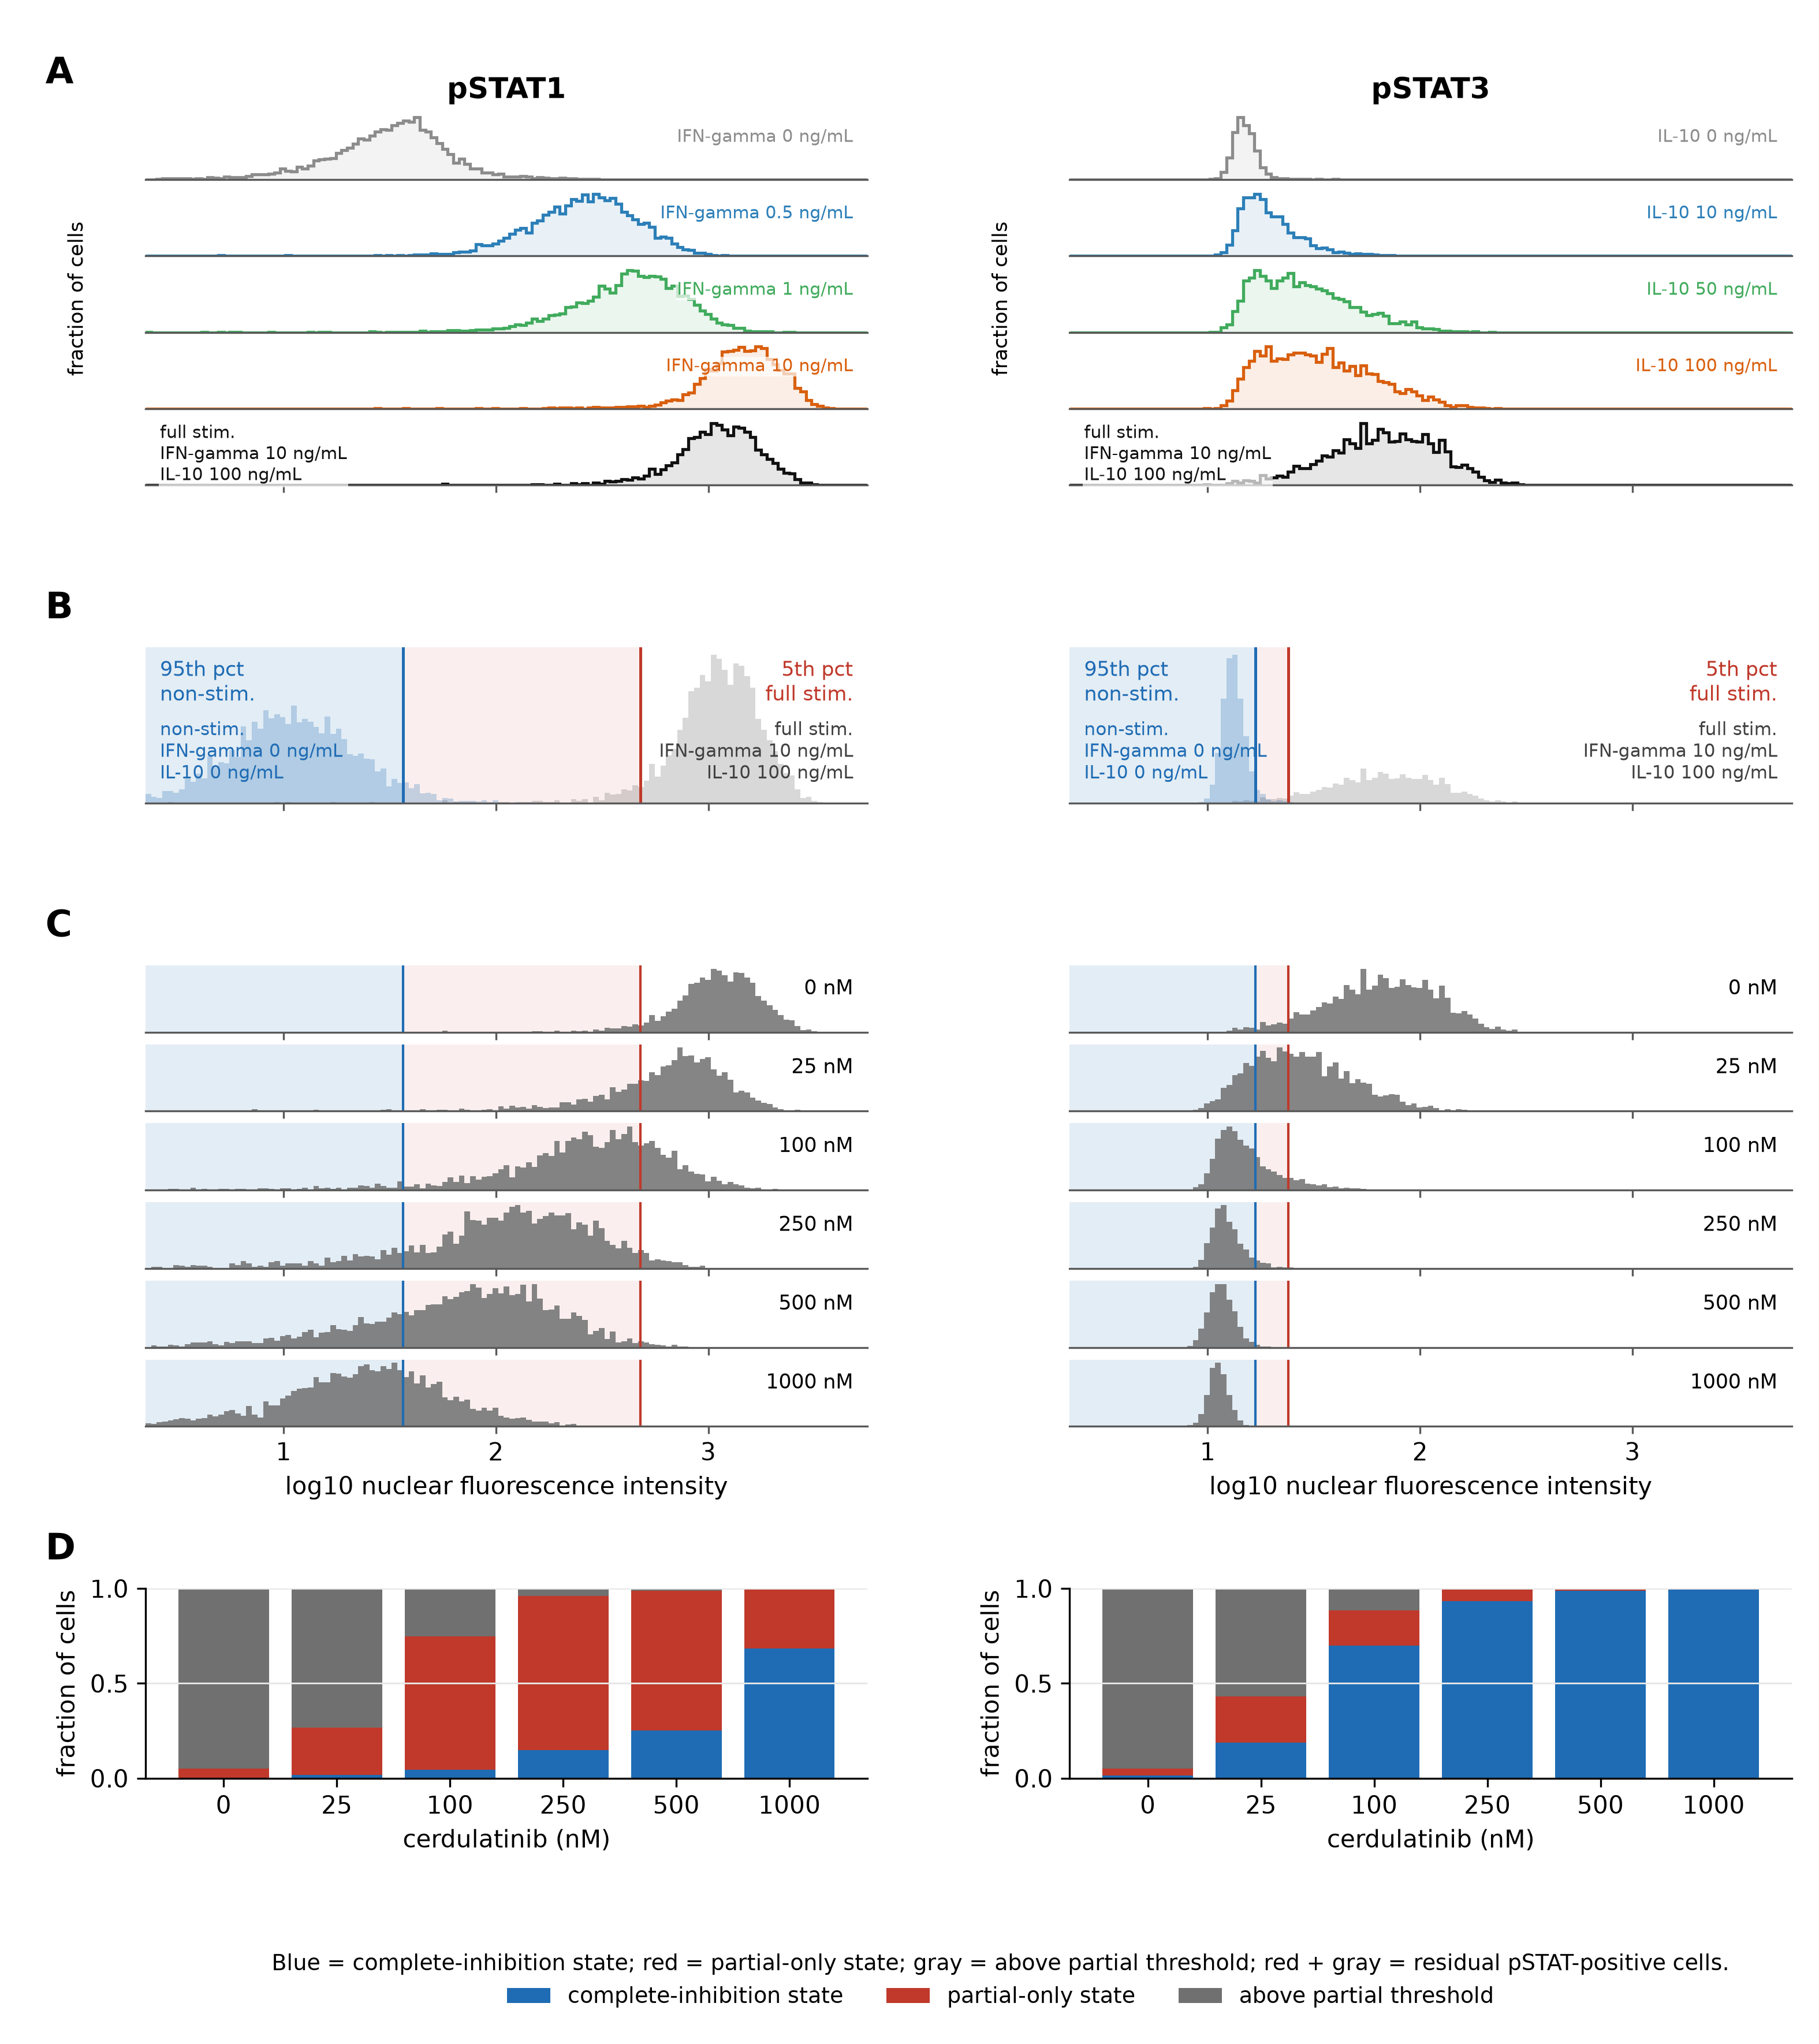
\includegraphics[height=0.70\textheight,keepaspectratio]{figures/Figure_1.png}
\caption{\textbf{Single-cell response distributions define reference states for inhibitor interpretation.}
(A) Nuclear \pstatone{} distributions at \ifng{} doses of 0, 0.5, 1, and 10 ng/mL (left), and \pstatthree{} distributions at IL-10 doses of 0, 10, 50, and 100 ng/mL (right), from top to bottom. The final row shows combined full stimulation (\ifng{} 10 ng/mL; IL-10 100 ng/mL). Rows are independently y-scaled.
(B) Reference distributions: the 95th percentile of the non-stimulated distribution defines the blue complete-inhibition range; the 5th percentile of the fully stimulated distribution defines the upper bound of the red partial-only range.
(C) Responses to increasing cerdulatinib doses after full stimulation, relative to the fixed thresholds in B.
(D) Corresponding occupancy: blue, complete inhibition; red, partial-only inhibition; gray, above the partial threshold. Red plus gray constitutes the residual pY-STAT-positive fraction. Measurements are pooled across available technical replicates of one biological replicate; a second independent replicate showed similar qualitative patterns.}
\label{fig:fig1}
\end{figure}

\begin{figure}[p]
\centering
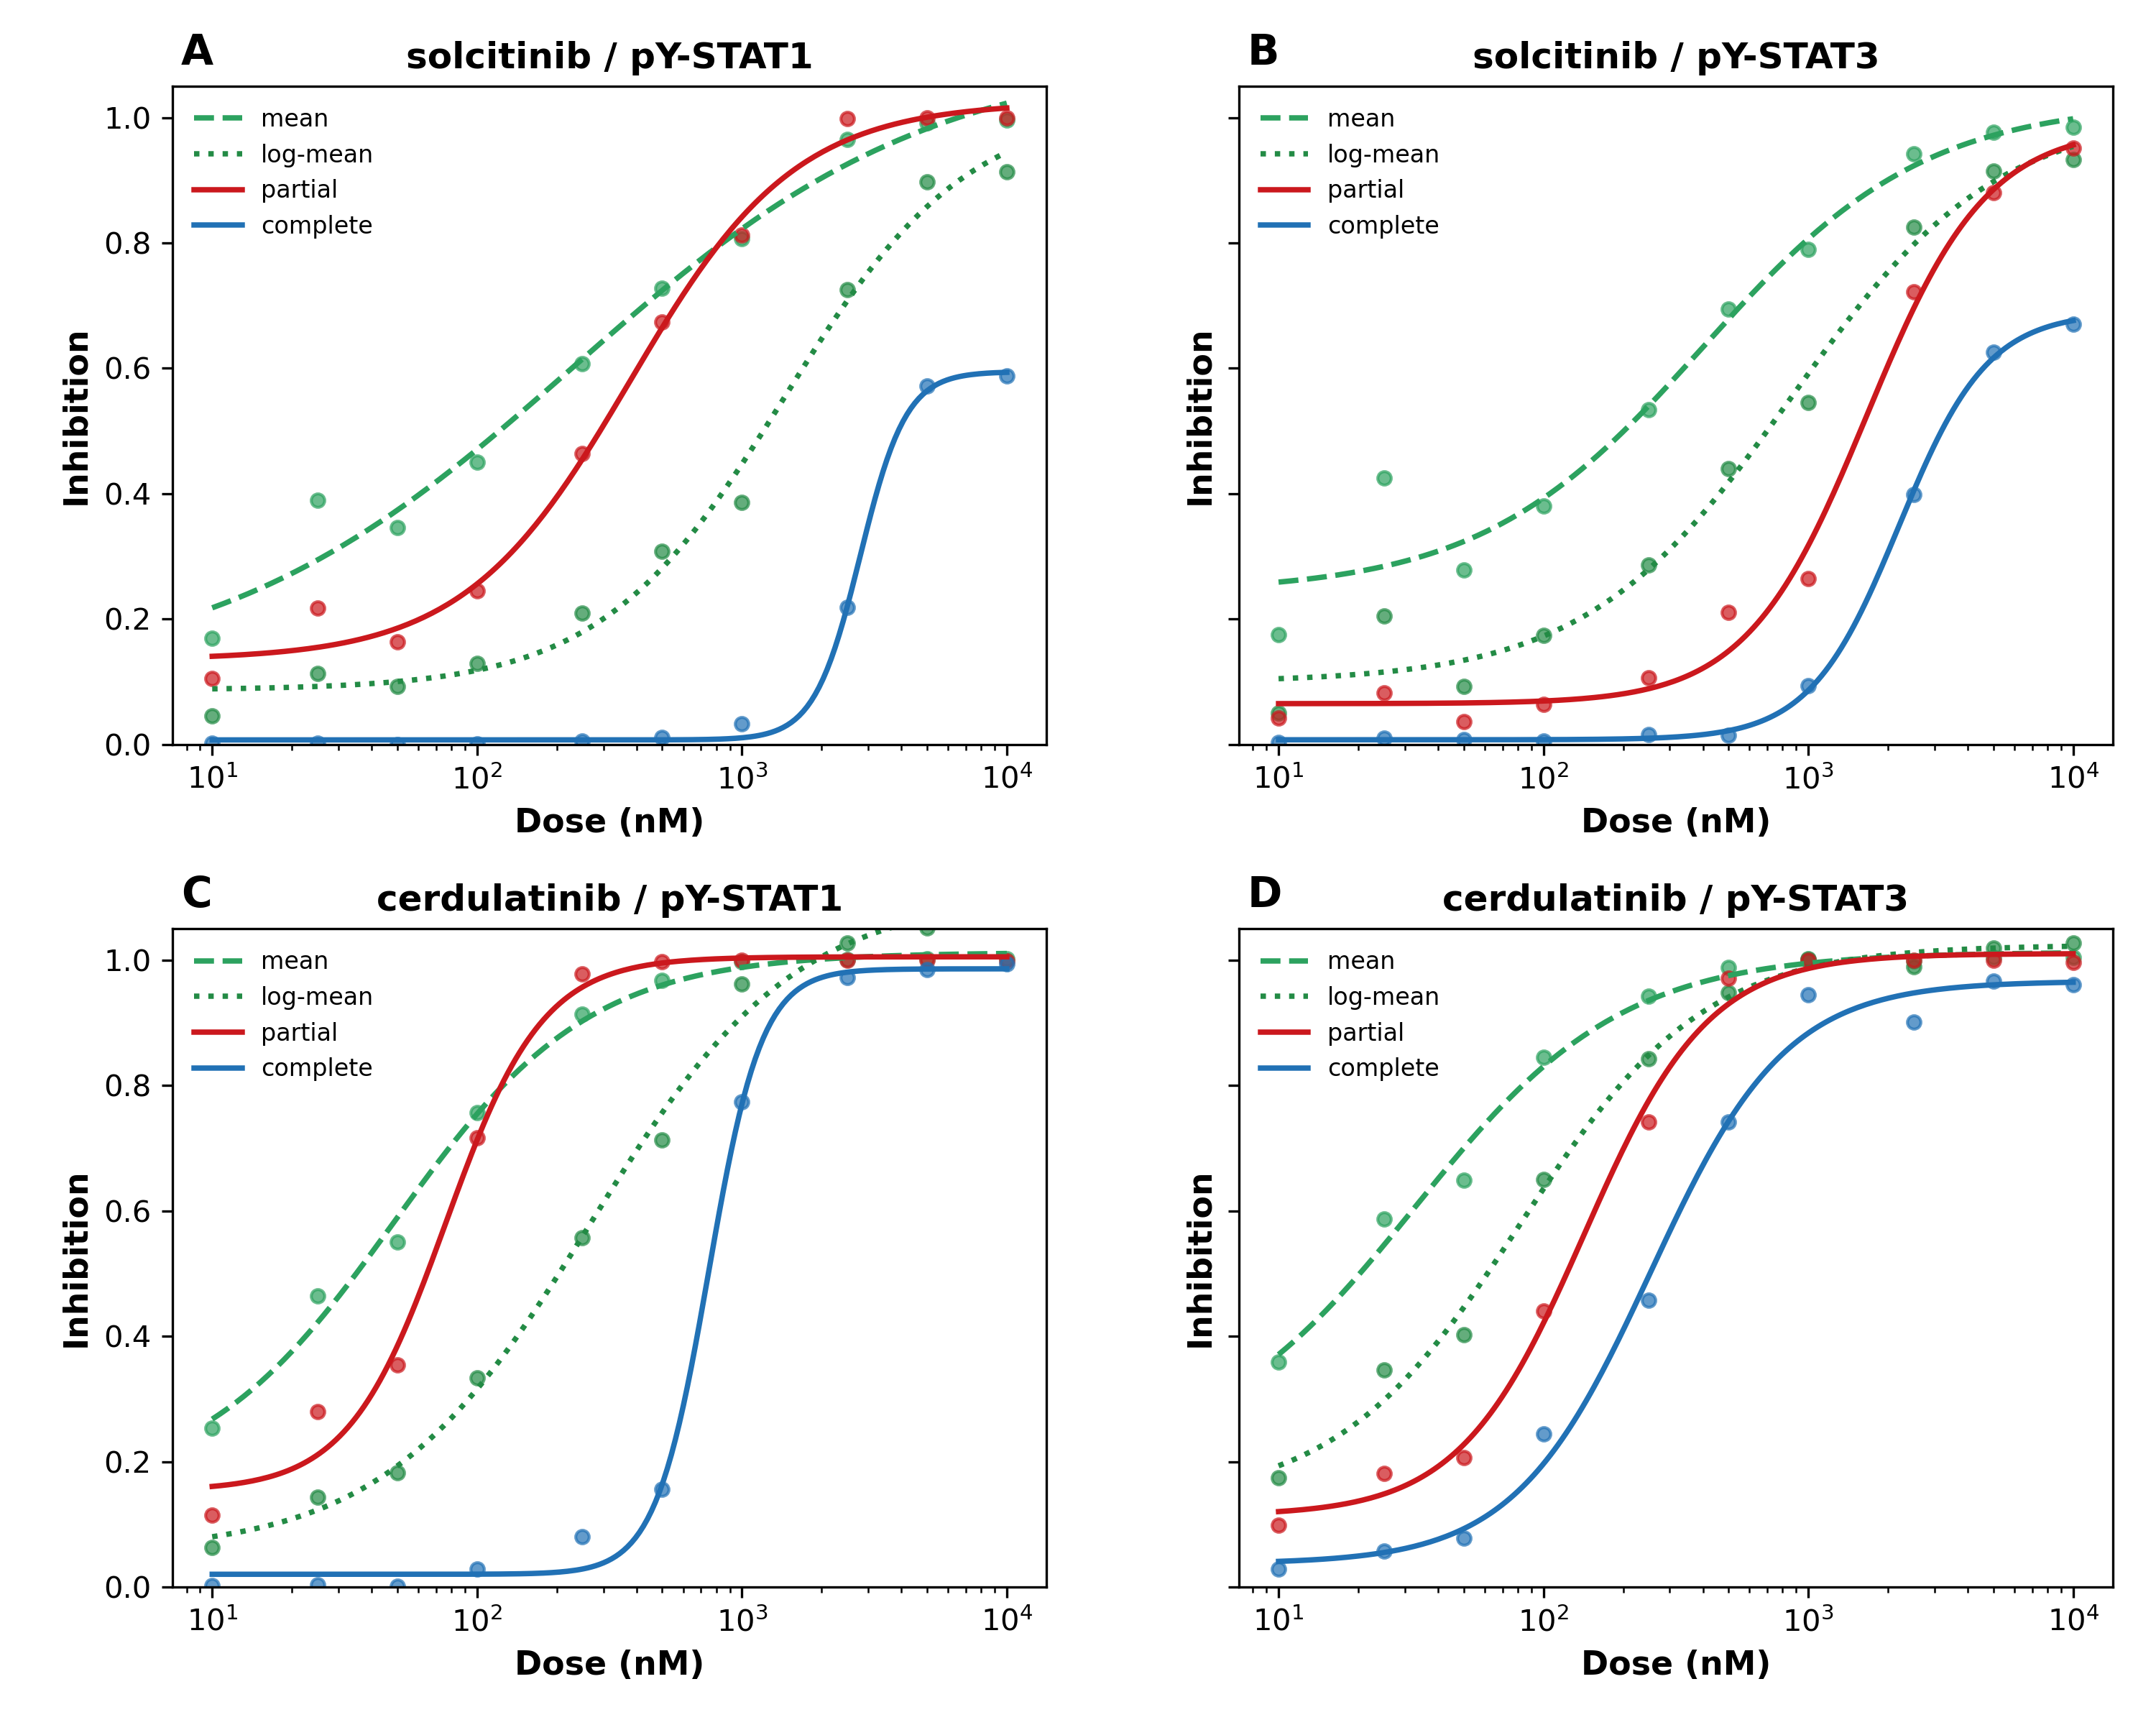
\includegraphics[width=\textwidth]{figures/Figure_2.png}
\caption{\textbf{Representative inhibition curves reveal dissociation between population suppression and state occupancy.}
Representative dose-response curves in THP-1 cells for solcitinib (A, B) and cerdulatinib (C, D), measured using \pstatone{} (A, C) and \pstatthree{} (B, D) as readouts after cytokine stimulation. Each panel shows four inhibition endpoints: arithmetic-mean inhibition, log-mean inhibition, partial-inhibition occupancy, and complete-inhibition occupancy. Points represent observed values at each inhibitor dose; lines show fitted dose-response curves. Arithmetic-mean inhibition provides the most left-shifted estimate of inhibition, log-mean inhibition shifts the population endpoint to higher doses, and complete-inhibition occupancy is generally the most right-shifted endpoint.
Points represent pooled observations from two technical replicates of one representative biological replicate, and fitted curves were generated from these pooled data; similar qualitative relationships were observed in a second independent biological replicate.}
\label{fig:fig2}
\end{figure}

\begin{figure}[p]
\centering
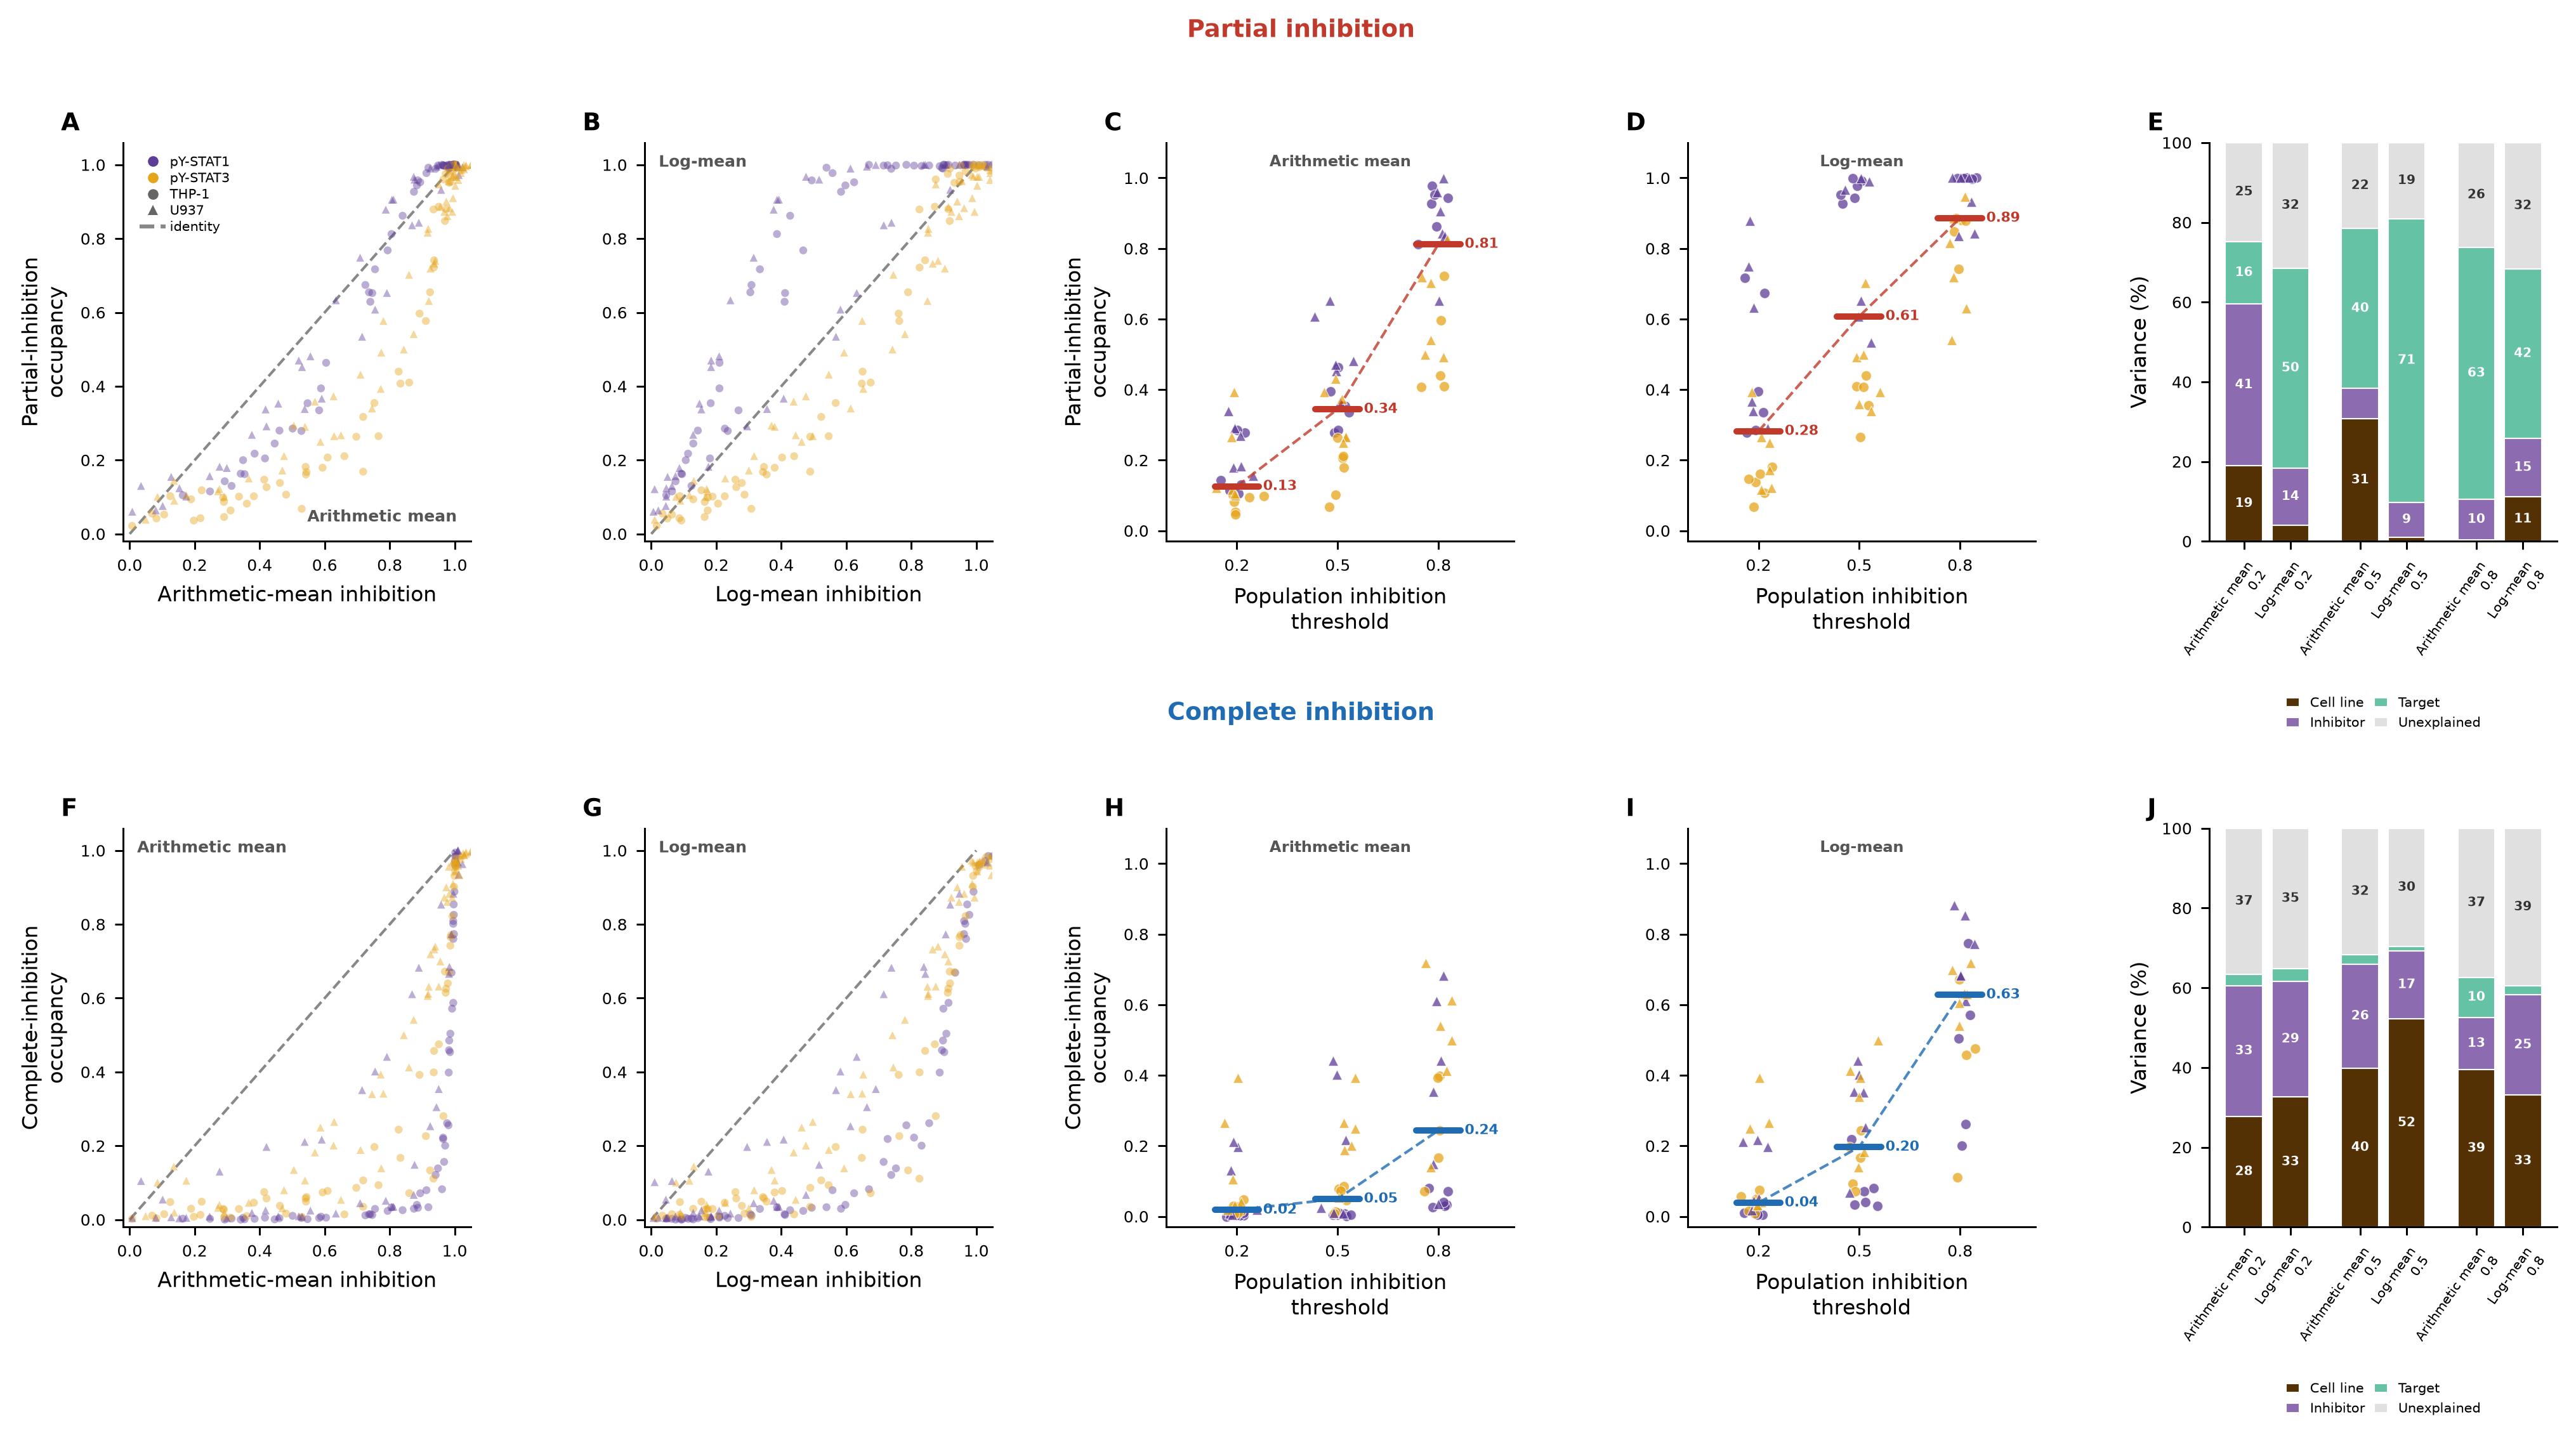
\includegraphics[width=\textwidth]{figures/Figure_3.png}
\caption{\textbf{Matching population inhibition to state occupancy quantifies residual pY-STAT-positive fractions.}
Partial-inhibition occupancy (A--E) is the fraction of cells below the fully stimulated response range; complete-inhibition occupancy (F--J) is the fraction within the non-stimulated response range. Violet and amber denote pY-STAT1 and pY-STAT3; circles and triangles denote THP-1 and U937.
(A, B) Partial-inhibition occupancy versus arithmetic-mean inhibition (A) or log-mean inhibition (B) at the same measured doses. Dashed line, identity. (C, D) Partial-inhibition occupancy at the lowest measured dose at which the fitted population-summary curve reached or exceeded 0.2, 0.5, or 0.8. Each point represents one profile; colored bars show medians and dashed lines connect them. (E) Descriptive variance shares associated with cell line, inhibitor, phospho-target, and an unexplained remainder for each benchmark and population summary (Methods).
(F, G) Complete-inhibition occupancy versus arithmetic-mean inhibition (F) or log-mean inhibition (G) at the same measured doses. (H, I) Complete-inhibition occupancy using the threshold-crossing procedure in C and D. At the 0.8 benchmark, median occupancy was 0.24 for arithmetic-mean inhibition and 0.63 for log-mean inhibition, leaving median residual pY-STAT-positive fractions of 76\% and 37\%, respectively. (J) Between-profile variance partitioned as in E. Cell line, inhibitor, and phospho-target together accounted for approximately 60--70\% of the variance; cell line was the largest identifiable contributor in most configurations and on average (label-permutation test, $p \le 0.003$). $n = 22$--24 evaluable profiles per benchmark; profiles whose fitted curve did not reach a benchmark were omitted.}
\label{fig:fig3}
\end{figure}

\begin{figure}[p]
\centering
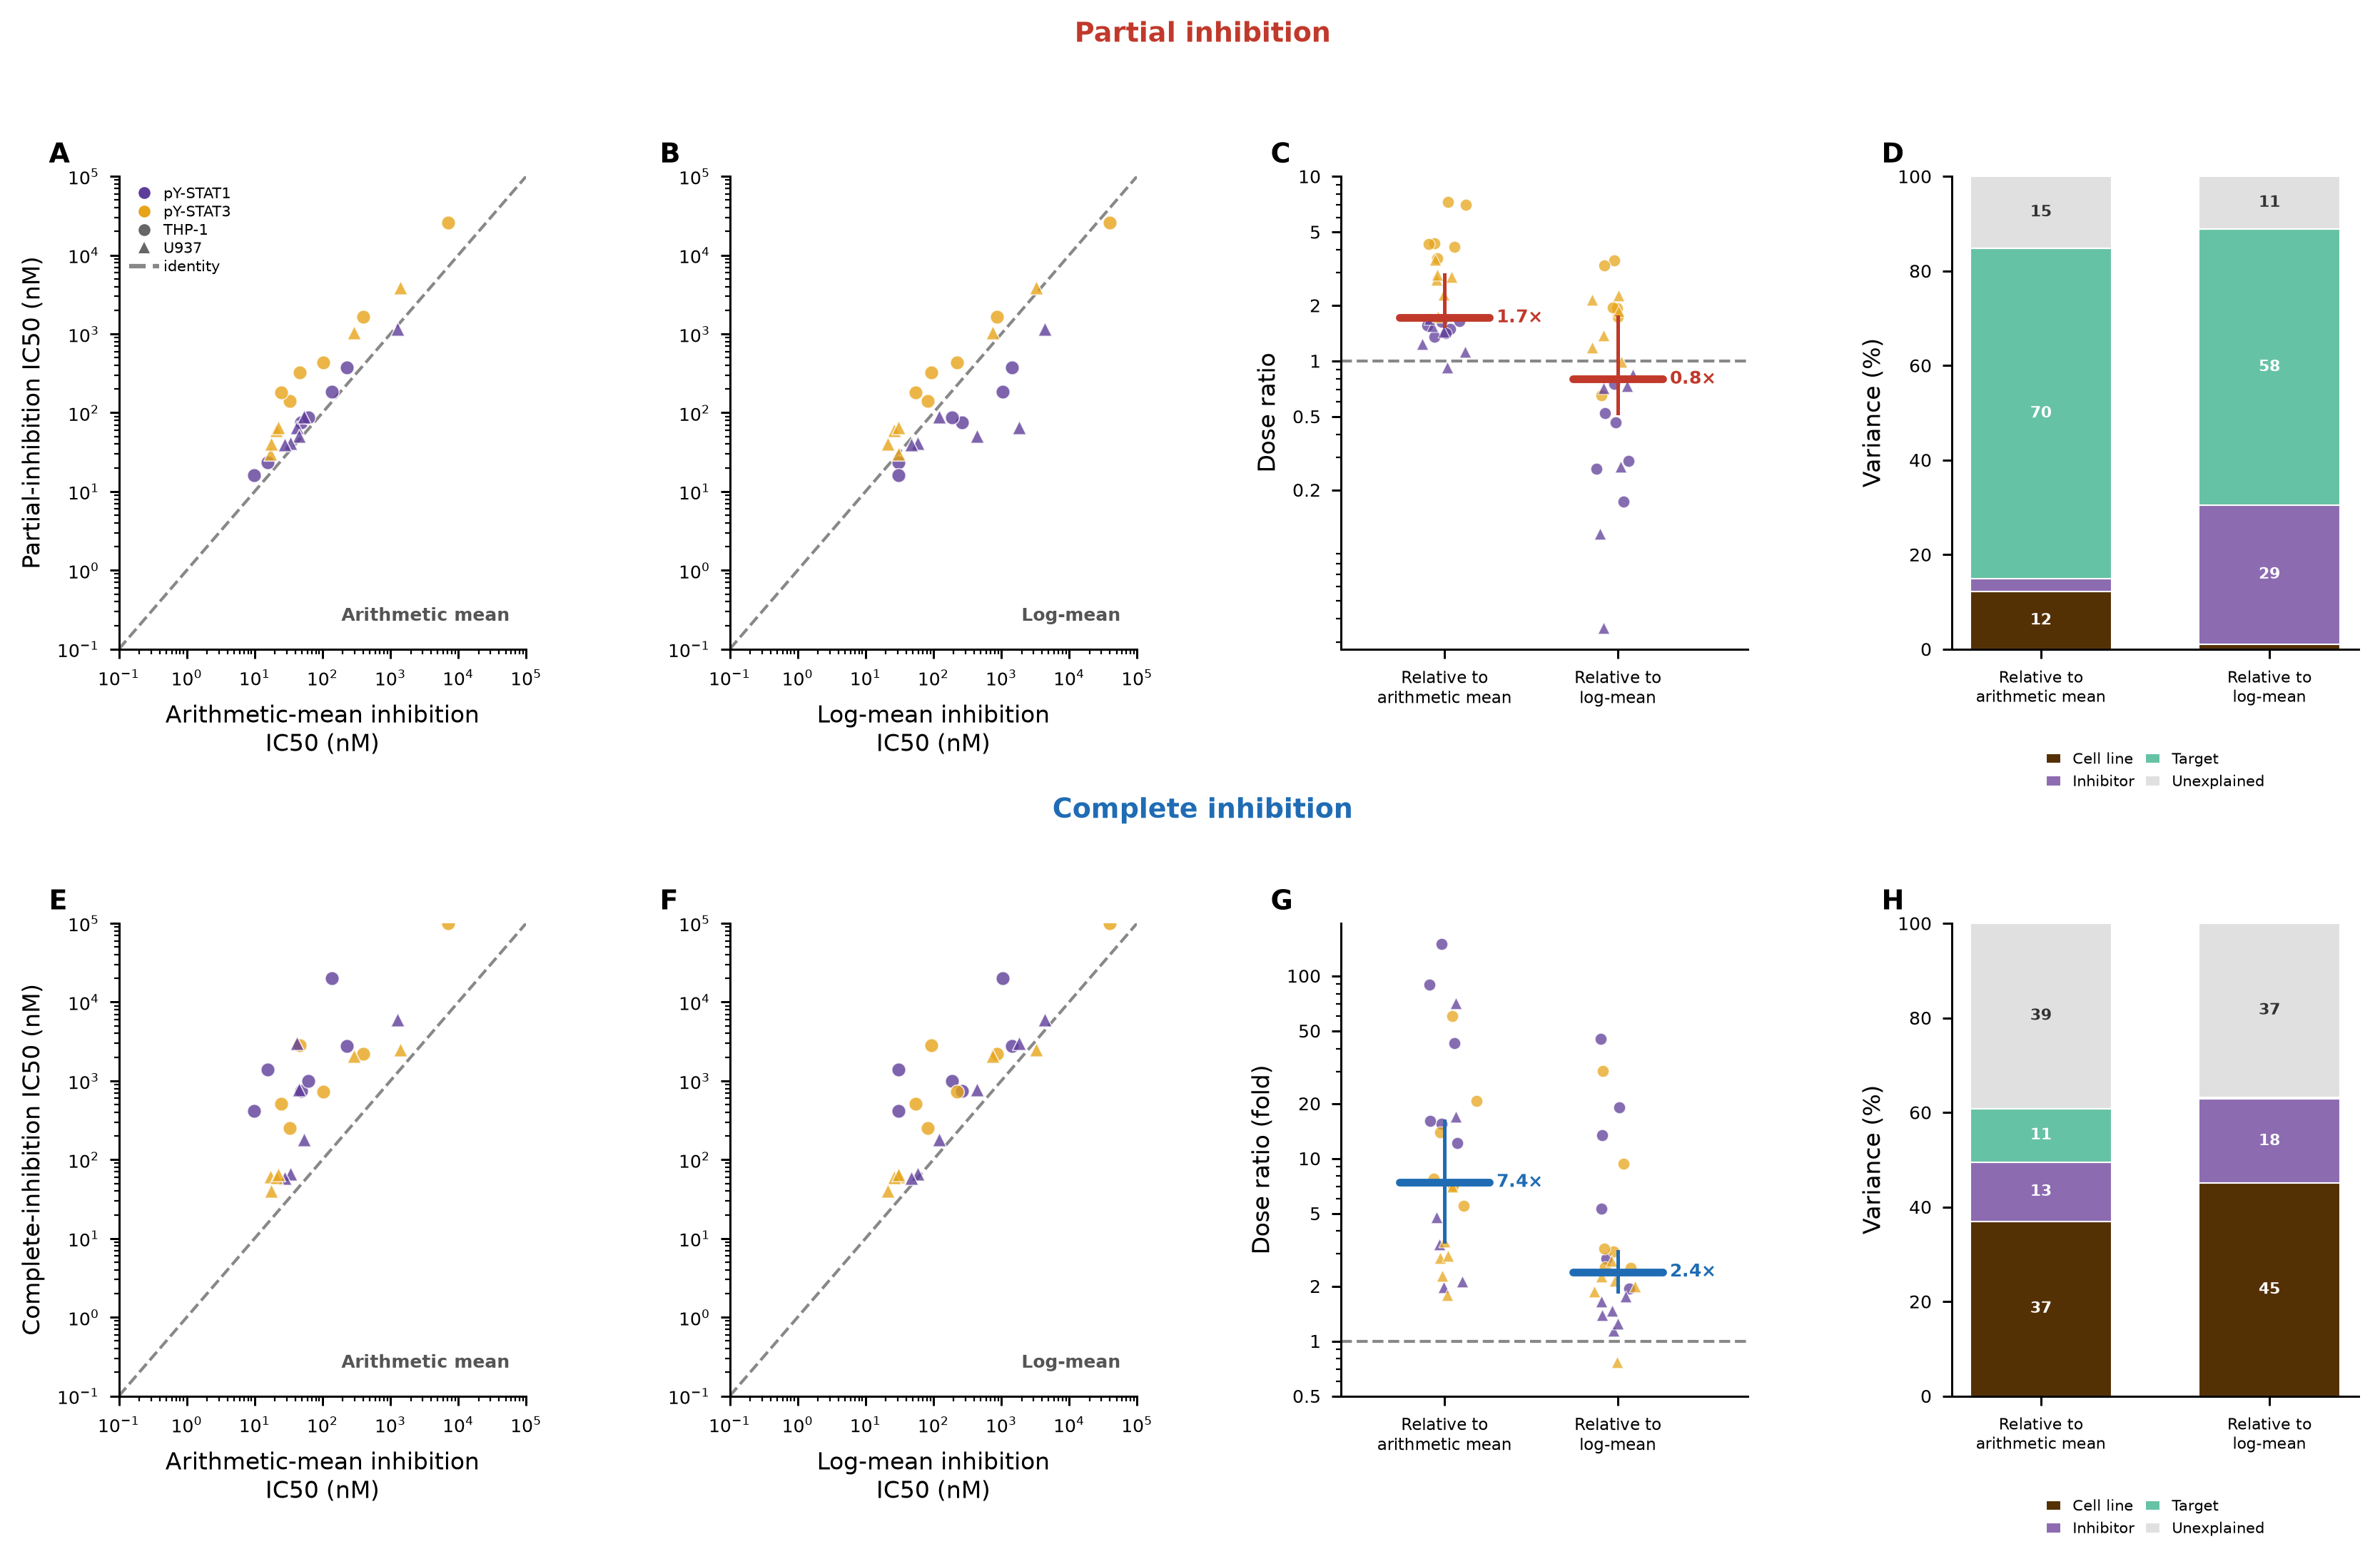
\includegraphics[width=\textwidth]{figures/Figure_4.png}
\caption{\textbf{Partial-inhibition \icfifty{} approximates log-mean \icfifty{}, whereas complete-inhibition \icfifty{} is right-shifted.}
The figure compares partial-inhibition occupancy (A--D) and complete-inhibition occupancy (E--H) with arithmetic-mean and log-mean inhibition across 24 inhibitor--cell-line--readout profiles. Violet and amber denote pY-STAT1 and pY-STAT3; circles and triangles denote THP-1 and U937.
(A, B) Apparent partial-inhibition \icfifty{} versus arithmetic-mean \icfifty{} (A) or log-mean \icfifty{} (B). Both axes are logarithmic; the dashed line denotes identity. (C) Per-profile ratios of partial-inhibition \icfifty{} to each population-summary \icfifty{}. Points show individual profiles, the horizontal colored bar denotes the median, the vertical line denotes its 95\% confidence interval obtained by bootstrap resampling of the 24 profiles (10{,}000 resamples), and the dashed line denotes a ratio of one. Median ratios were 0.8 relative to the log-mean (95\% confidence interval, 0.5--1.7) and 1.7 relative to the arithmetic mean (95\% confidence interval, 1.5--2.9). (D) Between-profile variance in the log10-transformed ratios from C, partitioned among cell line, inhibitor, phospho-target, and an unexplained remainder.
(E, F) Apparent complete-inhibition \icfifty{} versus arithmetic-mean \icfifty{} (E) or log-mean \icfifty{} (F), plotted as in A and B. (G) Per-profile ratios plotted as in C. Median ratios were 2.4 relative to the log-mean (95\% confidence interval, 1.9--3.1) and 7.4 relative to the arithmetic mean (95\% confidence interval, 3.5--16). (H) Variance in log10-transformed ratios from G, partitioned as in D. Factor shares are descriptive and do not separate cell line from batch; confidence intervals do not represent biological-replicate uncertainty (Methods).}
\label{fig:fig4}
\end{figure}

\clearpage
\section*{Supplementary figure legends}

\setcounter{figure}{0}
\renewcommand{\thefigure}{S\arabic{figure}}
\renewcommand{\figurename}{Supplementary Figure}

\begin{figure}[h]
\centering
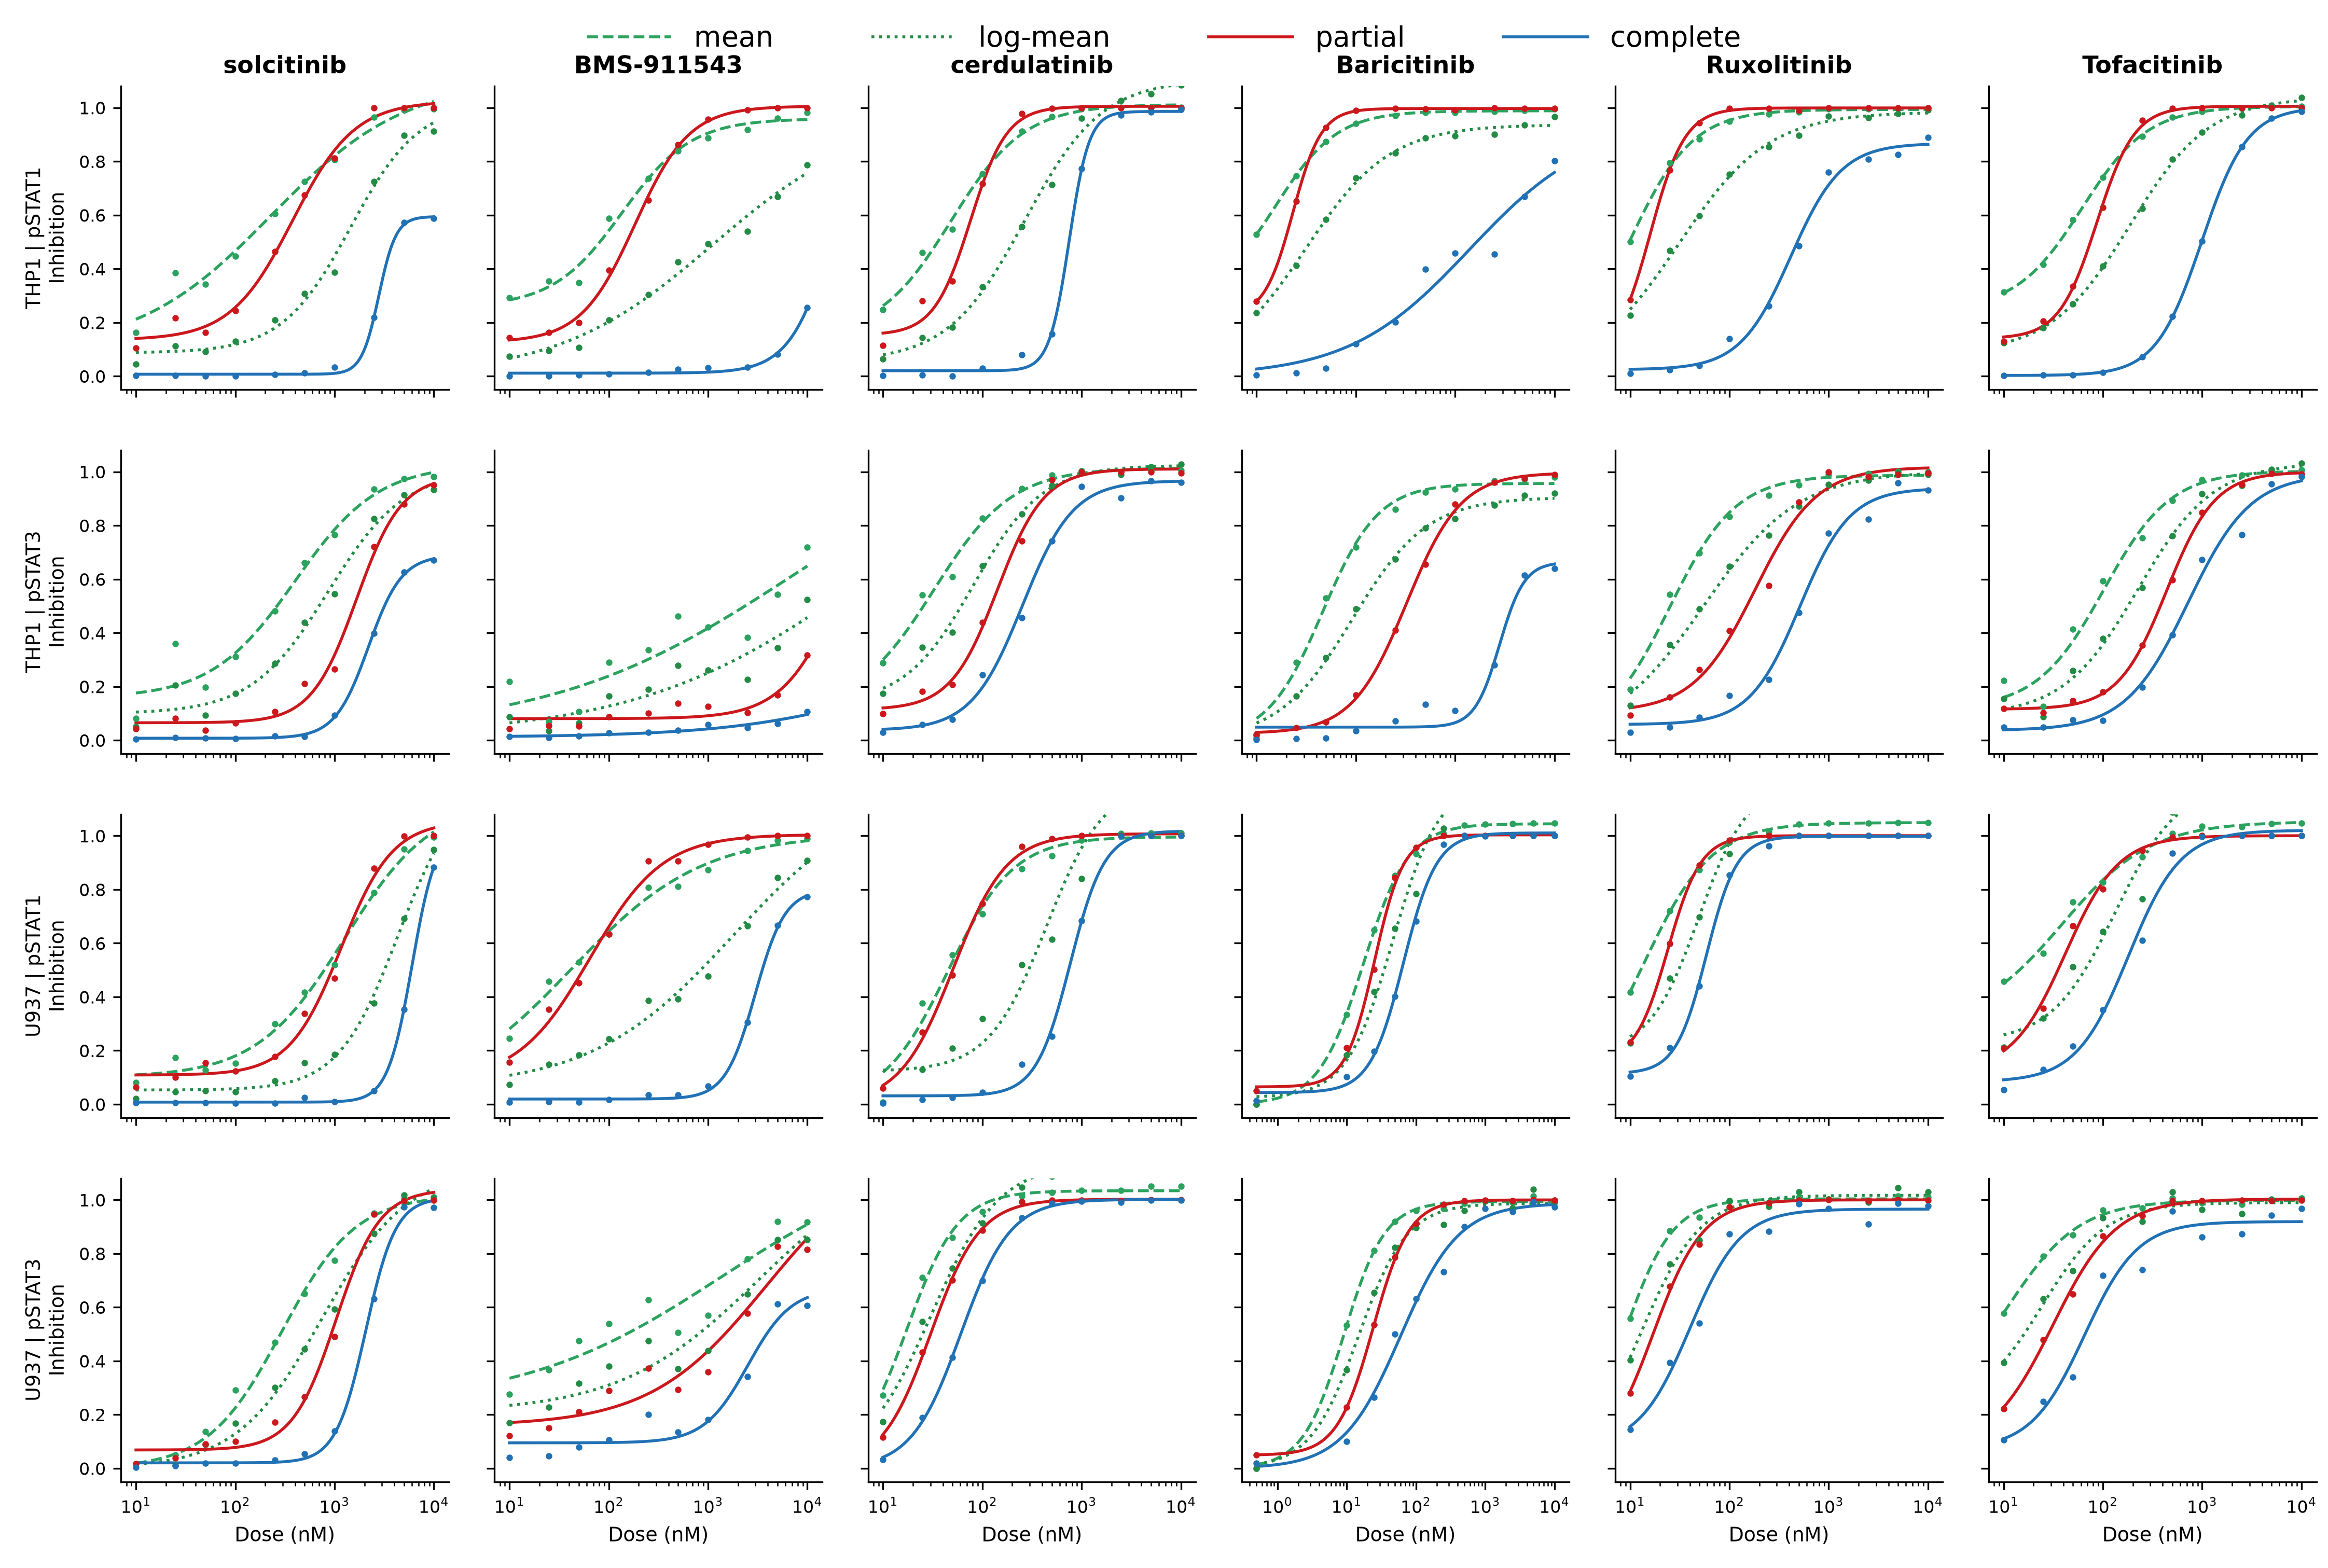
\includegraphics[width=\textwidth]{figures/Figure_S1.png}
\caption{\textbf{Full dose-response atlas across inhibitors, cell lines, and readouts.}
Observed inhibition values and fitted dose-response curves for arithmetic mean, log-mean, partial inhibition, and complete inhibition across all inhibitor--cell-line--readout combinations analyzed in this study. Columns correspond to the six inhibitors solcitinib, BMS-911543, cerdulatinib, baricitinib, ruxolitinib, and tofacitinib. Rows correspond to THP-1 \pstatone{}, THP-1 \pstatthree{}, U937 \pstatone{}, and U937 \pstatthree{}.}
\label{fig:figs1}
\end{figure}

\begin{figure}[h]
\centering
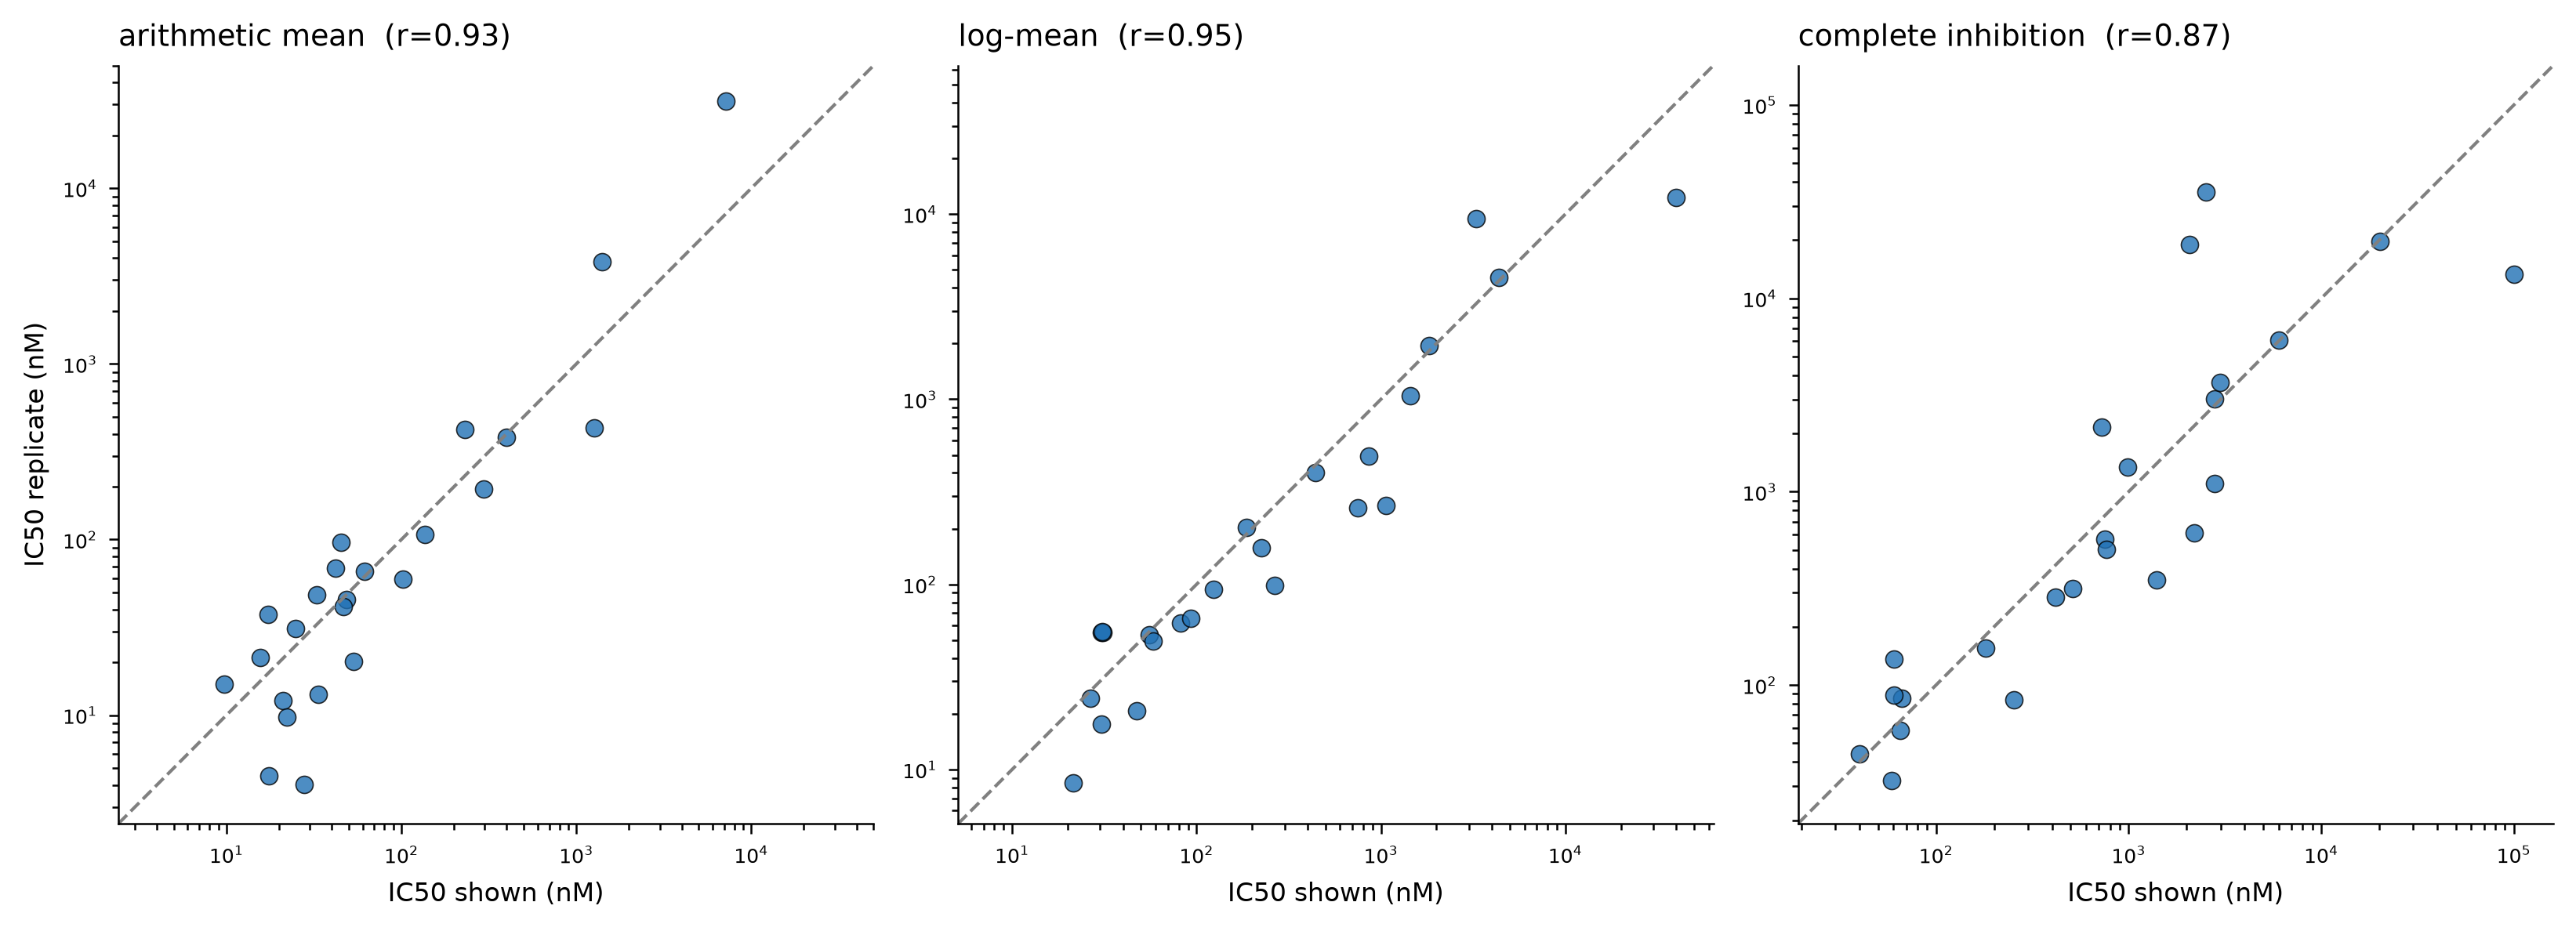
\includegraphics[width=\textwidth]{figures/Figure_S2.png}
\caption{\textbf{Comparison of apparent \icfifty{} estimates across biological replicates.}
For each of the four dose-response experiments, apparent \icfifty{} estimates from the deposited concordance table for the second biological replicate were compared with those of the representative replicate shown in the main figures. Each point is one inhibitor--cell-line--readout profile (24 profiles total); axes are shown on a logarithmic scale and the dashed line marks identity. Panels correspond to the arithmetic mean, log-mean, and complete-inhibition metrics; the log--log Pearson correlation is given in each panel title. The relative ordering of the metrics, including \icfifty{}(complete) exceeding \icfifty{}(log-mean), was preserved in the replicate dataset.}
\label{fig:figs2}
\end{figure}


\end{document}
